% !TEX TS-program = pdflatex
% !TEX encoding = UTF-8 Unicode

% This is a simple template for a LaTeX document using the "article" class.
% See "book", "report", "letter" for other types of document.

\documentclass[11pt]{article} % use larger type; default would be 10pt

\usepackage[utf8]{inputenc} % set input encoding (not needed with XeLaTeX)
\usepackage{graphicx}
\graphicspath{{images/}}
\usepackage{gensymb}
\usepackage[hidelinks]{hyperref}

%%% Examples of Article customizations
% These packages are optional, depending whether you want the features they provide.
% See the LaTeX Companion or other references for full information.

%%% PAGE DIMENSIONS
\usepackage{geometry} % to change the page dimensions
\geometry{a4paper} % or letterpaper (US) or a5paper or....
% \geometry{margin=2in} % for example, change the margins to 2 inches all round
% \geometry{landscape} % set up the page for landscape
%   read geometry.pdf for detailed page layout information

\usepackage{graphicx} % support the \includegraphics command and options

% \usepackage[parfill]{parskip} % Activate to begin paragraphs with an empty line rather than an indent

%%% PACKAGES
\usepackage{booktabs} % for much better looking tables
\usepackage{array} % for better arrays (eg matrices) in maths
\usepackage{paralist} % very flexible & customisable lists (eg. enumerate/itemize, etc.)
\usepackage{verbatim} % adds environment for commenting out blocks of text & for better verbatim
%\usepackage{subfig} % make it possible to include more than one captioned figure/table in a single float
\usepackage{amsmath}
\usepackage{caption}
\usepackage{subcaption}
% These packages are all incorporated in the memoir class to one degree or another...

%%% HEADERS & FOOTERS
\usepackage{fancyhdr} % This should be set AFTER setting up the page geometry
\pagestyle{fancy} % options: empty , plain , fancy
\renewcommand{\headrulewidth}{0pt} % customise the layout...
\lhead{}\chead{}\rhead{}
\lfoot{}\cfoot{\thepage}\rfoot{}

%%% SECTION TITLE APPEARANCE
\usepackage{sectsty}
\allsectionsfont{\sffamily\mdseries\upshape} % (See the fntguide.pdf for font help)
% (This matches ConTeXt defaults)
\setcounter{secnumdepth}{5}
%%% ToC (table of contents) APPEARANCE
\usepackage[nottoc,notlof,notlot]{tocbibind} % Put the bibliography in the ToC
\usepackage[titles,subfigure]{tocloft} % Alter the style of the Table of Contents
\renewcommand{\cftsecfont}{\rmfamily\mdseries\upshape}
\renewcommand{\cftsecpagefont}{\rmfamily\mdseries\upshape} % No bold!

%%% END Article customizations

%%% The "real" document content comes below...

\title{Face Tracking for Optimized Bitrate Control in Low Delay Video Encoding}
\author{Chethan Ningaraju}
%\date{} % Activate to display a given date or no date (if empty),
         % otherwise the current date is printed 

\begin{document}
\maketitle
\clearpage
\tableofcontents
\clearpage
%%%
%%%%INTRODUCTION
%%%%
\section{Introduction}
	In recent years, there is increasing demand for high-quality video conferencing solutions. Due to availability of high-speed and low-delay internet, video conferencing has proved to be an efficient alternative to face-to-face meeting. Video telephony has grown into a multi-billion dollar industry and has huge commercial significance. To address this growing need there has been constant improvement in  low-delay video coding techniques along with better techniques to ensure low-delay transmission reliability at the network level. The tremendous increase in smartphone usage has led to increase in video telephony over cellular networks whose bandwidth is highly constrained. Therefore, it is very important to develop methods of delivering high quality video with less bandwidth requirement. 

The most commonly used video coding standards like H.264/AVC have been designed to exploit the spatial and temporal redundancy in the input video stream to achieve high data compression. The techniques of spatial and temporal prediction forms the core principle of these video coding standards. However, after encoding the video the perceptual redundancies still remains, since human attention does not focus on the whole scene but only a small region of fixation called region-of-interest (ROI) \cite{Perception-model-of-face}. Therefore, reducing the perceptual redundancy gives a new dimension towards achieving lower bit-rate at acceptable perceptual quality.

The goal of this work is to identify the salient region of a frame, which is the face of the participant in a video conference. Since the attention of the viewer is mostly focused on the face of the other participants during a video conference call, improving the quality of the face region (ROI) can improve the overall perceptual quality. In this work, we assume ideal capture conditions and use the results of the face tracking directly as side information for the H264/AVC encoder's bitrate control. This work explores the methods of region of interest(ROI) based encoding to exploit the available bandwidth to encode regions that are of high importance to perceptual quality with higher quality. Face region in the input stream is allocated an above-average bit-count to yield a better visual quality than the background regions. It is also the aim of this work to develop and extensively evaluate the strategy of uneven bit-allocation and also to identify its limitations.

\subsection{ROI-based Coding}

In conventional video coding, all regions of a frame are considered equally important to the viewer. It is assumed that all regions contribute equally to the perceptual quality. However, the study of Human Visual System (HVS) shows that human eyes can only focus on one area in a frame at any given point in time which is called region of interest. For example, it has been found out in \cite{human-vision-proof-NSI} that humans normally perceive clearly a small region of 2–5\degree of the visual angle.

In video coding, the compression gains from spatial and temporal prediction is reaching saturation level. Further compression from these techniques demand exponential growth in computational capabilities. Therefore, perceptual coding can provide an efficient solution towards lower bitrate video coding. Some of the commonly used video codecs use the fact that high frequency components are less important to the human visual system and perform preferential coding based on spatial frequency. The higher frequency components which are not so important to the perceptual quality are encoded with higher QP. However, such preferential coding does not take into account the region of interest to the viewer in the frame to be encoded. All high frequency components are coded with higher quantization irrespective of the region belonging to ROI. 

The ROI-based coding is not a common practice in video coding because it is very hard to automatically detect important regions in generic contents that contribute the most to the perceptual quality. There are many ways of detecting region of interest, most of which are application specific. The most common approach is usage of difference image based moving object detector. In these systems any moving object is considered as ROI. A typical use-case for such a system is video surveillance. In addition to difference image based motion detection, global motion estimation is used in ROI detection \cite{ROI-aerial-surveillance} in applications like aerial surveillance.

In generic video content region of interest constantly keeps changing depending on the context. For instance, in a movie, the ROI can depend on context of the scene. Developing generic techniques for detection of ROI in such videos is very difficult. There have been attempts to use eye tracker to record the foveation points of a human observer on the receiver which was used to apply foveation filter in video coding of the sender. An advancement over such approach is proposed in \cite{foveated-rate-control} which optimizes rate control to maximize foveal visual quality metric. These generic ROI detectors are very hard to implement due to uncommon availability of eye tracking mechanism at the receiver. 

The region of interest in the video conferencing scenario is going to be the face region predominantly. Due to recent improvements in face detection algorithms it is possible to detect the face with good accuracy. The study in \cite{HighQualityROICodingForVideoConferencing} shows how boosting quality of the face regions can improve the overall perceived quality of the video. This work aims to study possible ways of improving perceptual quality of the video by detecting face region and coding it with higher quality than rest of the frame.

The knowledge of region of interest in input video can be used for many other purpose in addition to its use in video coding to improving perceptual quality. For instance, ROI information can be used in developing techniques for smart thumbnail display in group video conferencing solutions. In group video conferencing, an active person is detected based on the source of voice and is displayed on the main screen and other participants are displayed on the smaller windows with down-scaling of the entire video. If the face coordinates of the participant is transmitted along with the bit-stream as meta-data, a cropped version of video can be displayed to show only the face in thumbnail display. This can improve overall user-experience.

\subsection{Bitrate Control} \label{Intro:Bitrate-Control}
	The bitrate control module is responsible for controlling the bit-consumption of the encoder to guarantee smooth playback. Bitrate control is not video coding standard specific and operates independent of any chosen video coding standard. There are various flavors of bitrate control like Constant Bitrate (CBR), Variable Bitrate (VBR) and Average Bitrate (ABR). In this work, CBR type of bitrate control is considered since it is most commonly used in video conferencing and other real-time streaming applications. 
\begin{figure}[h]
    \centering
    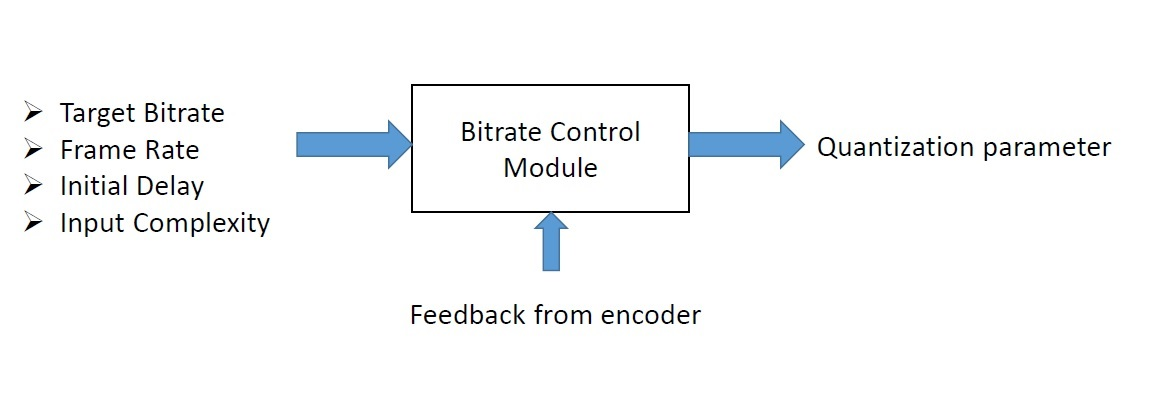
\includegraphics[scale=0.5]{RC_block}
    \caption{Bitrate Control Module Functionality}
    \label{fig:Bitrate Control Module Functionality}
\end{figure} 

\begin{figure}[h]
    \centering
    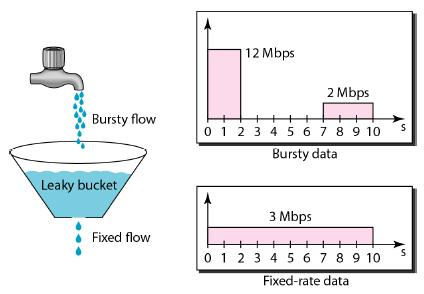
\includegraphics[scale=0.5]{general/Leaky_bucket}
    \caption{Leaky Bucket Model}
    \label{fig-Leaky-Bucket-Model}
\end{figure} 	
	Figure \ref{fig:Bitrate Control Module Functionality} illustrates the functionality of the bitrate control module. The main purpose of the bitrate control module is to ensure smooth playback of the encoded video under given bandwidth and delay constraints. It estimates the video bitrate based on the available network bandwidth, ensures the coded bitstream can be transmitted successfully and makes full use of the limited bandwidth \cite{InTech-Rate-control-in-video-coding}. It achieves this by controlling the quantization parameter (QP) used during the encoding. The quantization parameter is computed considering the input bitrate, framerate, input complexity (spatial and temporal activity) and acceptable delay of the system. The module also takes the feedback from the encoder regularly to make better QP decision.  The feedback from the encoder gives information about the content of the video and helps the bitrate control to compute right QP for a given bit-budget.
	
	The functionality of the Bitrate control module can be illustrated with the help of leaky-bucket model \cite{InTech-Rate-control-in-video-coding}. The output data-rate of a video encoder varies depending on the input complexity of the video (motion in the frame). It also depends on the picture type of the encoded frame. A frame can be encoded with spatial prediction (Key/I-frames), single direction temporal prediction (P-frames) and Bi-direction temporal prediction (B-frames). The key/I-frames consume a lot of bits compared to inter pictures (P-frames and B-frames). In a video streaming scenario considering a constant bitrate channel, the throughput is maximum when data-rate is constant and equal to the available bandwidth. Therefore, the output data of the encoder is smoothened using a theoretical buffer called Video Buffer Verifier (VBV). The VBV buffer is a virtual buffer modeled by the bitrate control module to ensure that video stream can be correctly buffered, and played back at the decoder end. This is equivalent to a leaky-bucket model as shown in Figure \ref{fig-Leaky-Bucket-Model} \cite{Leaky-bucket-NSI}, where the output of the encoder with variable rate (bursty output) is stored in a buffer (leaky bucket) which is draining at a constant rate.  Any underflow or overflow of this buffer causes glitch in the video streaming. To ensure that there is no VBV buffer overflow or underflow, encoder's quantization parameter is adapted on a macroblock level so that the maximum allowed bit-count for an encoded frame is not exceeded.

 A typical bitrate control allocates bits at every macroblock and adjusts the QP. In a simple approach one would try to distribute the bitrate evenly across all macroblocks in the frame. Since load efficiency is of high importance it is not advisable to do multi-pass encoding for optimal bitrate allocation. Therefore, over-allocation in one macroblock has to be compensated by under-allocation (using a higher QP) for neighboring macroblocks, regardless of the image content. However, a more intelligent allocation strategy should take the image content into account. Thus parts of the image with higher importance (ROI) should be given a higher share of the overall bit-count which results in higher visual quality. Background regions would get a lower proportion of the bit-count.

%% Section to throw light on other works in same field
\section{Related Work}

The concept of region of interest based encoding has been around for a while. The different approaches of using ROI information to improve perceptual quality can be broadly classified into following categories based on which stage of processing the ROI information is used.
\begin{itemize}  
\item Preprocessing - Blurring
\item Video encoding - During RDO, bitrate control
\end{itemize}
The input video stream can be directly altered based on the ROI information. Many pre-processing approaches are also used to directly reduce unimportant information by applying a non-uniform distortion filter in a scene. For instance, the image is divided into foreground (ROI) and background (non-ROI) and the non-ROI parts are blurred in \cite{ROI-background-blurring} to save bits during encoding. The work in \cite{pre-postprocessig-ROI-codec-independent} is an example for codec independent ROI encoding. It can work with any codec and arbitrary ROI detector. In this approach input video stream is modified only to contain relevant information. The non-ROI pixels are replaced such that these regions can be very efficiently compressed by the encoder. The non-ROI macroblocks are either replaced by corresponding block from the previous frame or a black block. The non-ROI regions are reconstructed with post-processing assuming zero motion vector. This approach is used in scenarios where non-ROI regions are mostly discarded completely at the receiver end.

In video encoding, multiple approaches exist to preferentially code ROI regions with higher quality at the cost of non-ROI regions. The ROI information can be directly used in rate-distortion optimization (RDO) during video encoding to alter the quality of ROI region. One such approach is presented in \cite{ROI-rate-control-H264} in which non-ROI macroblocks are encoded only using AMC-based modes (Active MB Concealment). The non-ROI macroblocks are encoded with only motion vector but no residual information. This creates a bias to choose larger distortion for non-ROI blocks to save bits during Lagrangian optimization.

A more common way of ROI encoding is by altering the rate control module to allocate higher bits to ROI regions. The work in \cite{ROI-bit-allocation-h264} proposes a bit-allocation and rate control scheme for enhancing regional perceptual quality using SSIM as the quality metric for distortion-quantization modeling. Statistical analysis is adopted to obtain the relation between SSIM of reconstructed MBs and corresponding QP (from 20 to 51 in this paper) after standard video coding.

The ROI-based encoding specific to video conferencing is proposed in \cite{ROI-MV-based-face-tracking} for H.263. This work proposes an algorithm to track face using motion-vector information. Once ROI is detected, it proposes modification of bit-allocation for both CBR and VBR mode of rate control. The QP for these blocks is predicted from the rate modeling of ROI and non-ROI blocks. The work described in \cite{Perception-model-of-face} goes a step further in face detection based ROI encoding schemes by enhancing finer facial feature to improve the perceptual quality in high-resolution HEVC encoding. In this approach, different weights are assigned to the background, face, eyes, mouth and nose regions which are in-turn used to alter quality by ROI-based adaptive CTU (Coding Tree Unit) partition structure for HEVC.

Most of the previous work concerned with modification of rate control to achieve better quality in ROI macroblocks deals with altering bit-allocation module. This work proposes ways of achieving ROI encoding in rate control modules that do not have explicit bit-allocation at the macroblock level. The previous works mentioned above proposes effective methods to create the quality difference between ROI and non-ROI. They do not throw sufficient light on determining optimal quality difference to achieve best perceptual quality. The goal of this work is also to come up with a guideline to determine optimal quality difference to achieve best perceptual quality.

%%section for detailed overview of bitrate control	
\section{Overview of Bitrate Control Module} \label{sec:used-bitrate-control-overview}
This section gives an overview of the low-delay bitrate control module used in this work. The need for extremely low end-to-end delay in video telephony puts additional constraints on video coding which results in compromise of video quality. During the low-delay video encoding, tools like bi-directional prediction (B-frames) are disabled. The usage of B-frames needs buffering of at least one frame. This adds on to overall latency of the system which is highly undesirable in video conferencing. The tolerable delay in video encoding is a direct measure of Video Buffer Verifier (VBV) buffer size. When the size of the VBV buffer is very low (due to low delay), there is less room to accommodate the variation in bitrate of the encoder. This implies that there can be minimum variation in the size of a frame irrespective of the content. Any wrong prediction of QP by the bitrate control module can have bad impact since there is no additional time available to re-encode the content with corrected QP. 
 
 The bitrate control module used in this work is a modified version of \cite{JVTF086}.  The bitrate control does a frame level bit-allocation based on fullness of the VBV buffer, followed by adapting QP at the macroblock level. The functionality of the bitrate control module can be divided into two parts:
\begin{itemize}  
\item Bit Allocation
\item QP Prediction
\end{itemize}

\subsection{Bit Allocation} \label{used-bit-allocation-overview}

The low-delay encoding mode does not favor usage of key frames at regular intervals and B-frames. Therefore, in steady state only P-frames are used in encoding video conferencing content. This makes frame level bit-allocation simpler since there is no need to consider relative complexity between different types of frames during frame level bit-allocation. The key-frame at the beginning is handled using special cases.  

As depicted in Figure \ref{fig:Bitrate Control Module Functionality}, one of the inputs for bitrate control module is a delay/latency parameter (L). This is defined as the maximum permissible delay allowed between the encoder and the decoder assuming zero transmission delay. In other words, the delay parameter is the maximum allowed time for any encoded frame to be transmitted completely through a constant bandwidth channel of per-defined bitrate. In this work, delay parameter (L) is configured as,
\begin{equation} 
	L_0 = 165 ms \text{	and	} L = \frac{1.5 * 1000}{framerate}.
\end{equation}
Initially a delay of $L_0 = 165ms$ is allowed for the key-frame. This allows, allocation of higher than average bits for the key-frame. However, the delay parameter (L) for P frames in steady state is only 1.5 times the frame sampling delay. For instance, if the input video is sampled at 30 frames/sec, then the time interval between two consecutive frame is 33ms (frame sampling delay), the permissible delay(L) for frames in steady state is approximately 49ms. The usage of different delay values for first key frame and steady state P-frames is handled by changing the delay value gradually. The large key-frame at the beginning results in huge delay (165ms), this delay is gradually reduced by using less than average bit-count for subsequent few frames (half of average bit-count per frame). Once the over-consumption of first-key frame is compensated, the steady state delay of $49ms$ is maintained for rest of the sequence.

It should be noted that the initial delay in the system can only be reduced by displaying the initial few P-frames at shorter intervals than the time interval in which they were captured. This results in momentary increase in playback speed. In practical implementation, usage of above average bit-count for I-frame results in few dropped frames subsequently even if I-frame over-consumes marginally. All the above artifacts are considered as an acceptable trade-off to achieve good initial spatial quality by allocating huge amount of bits to the first key-frame.

The bit-allocation module uses VBV buffer fullness and delay parameter (L) to compute the bits allocated for the current frame to be encoded. The VBV buffer fullness before encoding $nth$ frame ($d_0^{n}$) is calculated based on the size of the previously encoded $(n-1)th$ frame in bits ($FrameSize_{n-1}$) as follows,

\begin{equation}
\label{Eq:Frame level bit error accumulation}
d_0^{n} = d_0^{n-1} + (FrameSize_{n-1} - AvgBitsPerFrame),
\end{equation}
$$ d_0^{n} = max(d_0^{n} , 0), $$
where $$ AvgBitsPerFrame = \frac{bitrate}{framerate}.$$

The allocated bits for the $nth$ frame is maximum amount of bits that can be transferred along with residual bits in the VBV buffer in the duration L ($49ms$ in the above example). The maximum acceptable delay in ms (L) is translated to bits using below equation,
$$ L_{bits} = \frac{L * birate}{1000}.$$
Therefore, allocated bits for current frame $(B_{alloc})$ is given by,
\begin{equation}
	\label{Eq:bit-allocation}
	B_{alloc} = L_{bits} - d_0^n .
\end{equation}
In practice, rate control QP predictions are not very accurate to exactly consume the bits that was allocated to the frame ($B_{alloc}$). If a frame consumes more bits than $B_{alloc}$, it violates the delay conditions. The encoded frame will be unable to reach the decoder in time with available bitrate. Hence, the frame is not added to the bitstream. These frames which are encoded but not part of the output of the encoder are called \textit{dropped frames}. Such dropped frames must be avoided since it causes jerky playback. A small room for inaccuracy of the QP prediction is considered at the end of the bit-allocation stage to avoid dropped frames. In practice, the target bits for QP prediction is slightly lesser than $B_{alloc}$ to avoid dropping the frame in case of marginal over-consumption of bits.

%%In code, the upper limit of buffer is some fraction of the VBV buffer, check it if this needs to be included
\subsection{QP Prediction}  \label{used QP prediction overview}
  Due to low VBV buffer size, the bitrate control needs to have very quick reaction to any deviation in bitrate to avoid dropped frames. The bitrate control algorithm computes the QP for every macroblock. The two factors considered while computing QP for a macroblock are:
  
\begin{itemize}  
\item Macroblock Complexity
\item Bitrate Deviation
\end{itemize}
\subsubsection{Macroblock Complexity}	
	Firstly, a delta QP (dq) is calculated considering the complexity of the macroblock. The activity of the macroblock is a measure of complexity of the macroblock and hence indicates the bits required to encode the macroblock. After motion compensation with the selected coding mode and motion vectors, the activity of a macroblock with index $(i,j)$, original pixel value $s(i,j)$ and predicted pixel value $c(i,j)$ is calculated using (\ref{Eq:activity_calc}). 
\begin{equation}
	\label{Eq:activity_calc}
	act_m = \sum_{i,j} \mid s(i,j)-c(i,j) \mid ,\quad	i,j = 1,2,....16.
\end{equation}	
	 The relative complexity of the macroblock with respect to the entire frame complexity is used in QP adaptation. The ratio of activity of the current macroblock and average activity of the entire frame is used to calculate the delta QP (\ref{Eq:deltaQP}).
\begin{equation}
	\label{Eq:deltaQP}
	dq = \begin{cases}
		-floor(\frac{avj\_act} {act_j} - 1), &  0 < \frac{act_j}{avg\_act} <= 1/2.\\
		0, & 1/2 < \frac{act_j}{avg\_act} <= 2.\\
		floor(\frac{act_j} {avj\_act}) - 1, & \frac{act_j}{avg\_act} >= 2
	\end{cases}
\end{equation}
As depicted in the above equation, a positive dq is used when current macroblock is relatively more complex compared to average frame complexity. This indicates that for relatively complex macroblocks within a frame, a higher QP is used. This is to make sure that bits within a frame is equally distributed across all the macroblocks. Such activity based QP adaptation results in uneven quality within a frame. The peak signal to noise ratio (PSNR) of the simple or static region is higher than that of regions with high motion (foreground). In practice, the average frame activity of the entire frame is unavailable until the last macroblock of the frame has been encoded. Therefore, previous frame average activity is used as current frame activity since the two adjacent frames in a video are likely to remain similar. 

The activity metric used in (\ref{Eq:deltaQP}) is a complexity metric, hence it can be replaced by similar metrics depicting the complexity of the block. Other metrics like SATD (Sum of Absolute Difference in Transform Domain) calculated similar to activity calculation in (\ref{Eq:activity_calc}) and cost of the macroblock (J) can be used instead of the activity. In this work, cost of the macroblock computed during rate-distortion optimization (\ref{Eq:CostCalc}) is used as the complexity metric. 
 \begin{equation}
	\label{Eq:CostCalc}
		J = D + \lambda R.
\end{equation}
Here the distortion D represents the residual error after prediction measured as the sum of absolute difference (SAD) of original block and reconstructed block, is weighed against the number of bits R associated with motion information using the Lagrange multiplier $\lambda$. The least cost of all the evaluated modes is considered as the complexity of the block. The cost of the macroblock factors in both the amount of residual information to be encoded after motion compensation and bits used for signaling the mode and the motion vector. This makes it more accurate in terms of reflecting the complexity of the block compared to activity computed in (\ref{Eq:deltaQP}).
\subsubsection{Bitrate Deviation} \label{sec: Bitrate overview: Bitrate deviation}
	The delta QP ($dq$) calculated above is added to the QP calculated based on the deviation in the bitrate reflected by instantaneous VBV buffer fullness. The buffer fullness corresponds to fullness of the VBV buffer discussed in the context of leaky bucket model in section \ref{Intro:Bitrate-Control}. Any deviation in bitrate will be reflected in the occupancy of the buffer. For example, a higher level of buffer indicates over-consumption of bits. The VBV buffer occupancy ($d_0^n$) is calculated only after entire frame is encoded. In order to account for the deviation in bitrate at macroblock level, a global deviation factor is computed at the macroblock level based on the deviation in frame level bit-consumption of past frames and size of the macroblocks encoded in the current frame. The global deviation factor ($D_m^{n'}$) when encoding the $m^{th}$ macroblock of $n^{th}$ frame is calculated using (\ref{Eq:buffer_fullness}).
\begin{equation}
	\label{Eq:buffer_fullness}
	D_m^{n'} = d_0^{n'} + CurFrameBitCount - \frac{B_{alloc} * m}{M}.
\end{equation}
%%WARNING - The global deviation factor and VBV buffer fullness do not just differ by clipping, but also with different init value	
Here M is the total number of macroblocks in a frame, $B_{alloc}$ is the bits allocated to the frame by bit-allocation module in (\ref{Eq:bit-allocation}) and hence remains a constant for the given frame. CurFrameBitCount is the bit-consumption of the current frame until the last encoded macroblock. The term $d_0^{n'}$ in (\ref{Eq:buffer_fullness}) is accumulated frame level bit-deviation which is computed similar to VBV buffer fullness ($d_0^n$). Since the VBV buffer fullness ($d_0^n$) is computed only after fully encoding the frame, the factor $d_0^{n'}$ also remains constant for a given frame. The two terms $d_0^{n'}$ and $d_0^n$ differ with initialization values at beginning of the encoding \cite{JVTF086}. The frame level deviation factor ($d_0^{n'}$) is additionally subjected to clipping as shown in (\ref{Eq:DevClip}) after encoding every frame. 

The global deviation factor ($D_m^{n'}$) accounts for deviation in the bitrate of the encoded video until the last encoded macroblock. The global deviation factor is used to calculate QP parameter for the $m^{th}$ macroblock ($Q_m$) using (\ref{Eq:mainQP}).
\begin{equation}
	\label{Eq:mainQP}
	Q_m = \frac{D_m^{n'} * 31}{r} + dq,
\end{equation}
where
\begin{equation}
 r = i * bitrate/framerate \nonumber.
\end{equation}
The factor $dq$ in (\ref{Eq:mainQP}) is the delta QP computed using (\ref{Eq:deltaQP}). The factor $r$, is called the reaction factor. This factor indicates the number of frames over which the deviation in bitrate is to be compensated. The bitrate control module in this work uses $i = 1$.

%%Explain how bitrate is met
The working of bitrate control can be understood by analyzing the deviation factor $D_m^{n'}$ in (\ref{Eq:mainQP}). At the beginning of the frame (m = 0), $$D_m^{n'} = d_0^{n'}.$$ 
The allocated QP($Q_m$) solely depends on $d_0^{n'}$ if the deviation in macroblock level bit-consumption and activity based delta QP(dq) are ignored. The init value of $d_0^{n'}$ is chosen heuristically at the start of encoding based on the most used configuration. Therefore, the QP calculated for the first frame is not content dependent. Once the first frame is encoded, the bit-consumption usually differs from allocated bits by a large extent. For instance, if the content was more complex than average, the initial QP allocation will result in large bit consumption, increasing the value of frame level bit deviation ($d_0^{n'}$) which results in large global deviation ($D_m^{n'}$). This will result in larger QP value for next frame to be encoded according to (\ref{Eq:mainQP}). Therefore, the value of $d_0^{n'}$ oscillates for the first few frames. In steady state it takes optimum value to keep the deviation low eventually helping in meeting the bitrate. The frame level bit-deviation $d_0^{n'}$ is clipped between pre-computed maximum and minimum value to keep QP limit in a suitable range.
\begin{equation}
\label{Eq:DevClip}
d_0^{n'} = clip(1000, \frac{40 * r}{31})
\end{equation}

The QP output by rate control ($Q_m$) is clipped between valid range of QP in H.264 encoding. In addition to these limits, the QP computed in (\ref{Eq:mainQP}) is subjected to swing restrictions. Since the QP is modulated based on the activity of the macroblock, a upper limit of maximum QP ($QP_{max}$),
\begin{equation}
	\label{Eq:QP swing restriction}
	QP_{max} = QP_{avg} + 5,
\end{equation} 
is set to make sure the high activity regions are not excessively penalized with higher quantization. Here, $QP_{avg}$ corresponds to average QP of all the blocks in the previous encoded frame.

\section{Study Setup}
This section describes the the setup used in this work. It describes the configuration of the encoder used to evaluate different algorithms. It also describes the metrics and aspects used to benchmark the proposed ROI-based bitrate control algorithm against the state of the art bitrate control algorithm.
\subsection{Encoder Configuration} \label {sec:Encoder configuration}     
This work uses Citrix h264 video codec for the study. The encoder is configured in low delay mode suitable for video conferencing and other real-time applications. The bitrate control described in section \ref{sec:used-bitrate-control-overview} is used to control the output data-rate of the encoder. The encoder is configured to use IPPP mode with key/I-frame used only at the beginning of the sequence followed by only uni-directional P frames. Due to low delay there is no provision to re-encode the frame in case of buffer overflow. The frames are dropped entirely in case of buffer overflow to maintain a constant low-delay.

\subsection{Measurements}
One of the crucial aspects in this study is the metric used to evaluate various algorithms in order to choose the best approach. The goal of this study is to improve the quality of the ROI macroblocks at the cost of degrading the non-ROI macroblocks. Since the whole approach is to measure the gain in perceptual quality, using frame level PSNR alone as a metric could be misleading. 

In this study, the difference in average PSNR of frames and average ROI PSNR is used as one of the metrics to evaluate different algorithms. The expectation is to see an improvement in ROI PSNR, with degradation in PSNR of the non-ROI regions. The shift in quality of ROI and non-ROI parts should be achieved keeping the bitrate unchanged. Therefore, the second aspect is to measure the deviation in bitrate behavior with ROI-based encoding compared to normal encoding without using any ROI information. Third aspect involves the measurement of PSNR and QP distribution within a frame. The QP distribution helps in analyzing the preferential QP computation for ROI regions which reflects in the form of below-average QP used in ROI. The PSNR distribution within a frame is studied to ensure that there is visible improvement in the quality of ROI without badly degrading the quality of the non-ROI. 

To measure all these behaviors following metrics are considered
\begin{itemize}  
\item Quality metrics - PSNR of ROI and non-ROI regions.
\item PSNR and QP variation within a frame.
\item Delay plot comparison for the entire sequence.
\end{itemize}
\subsubsection{Quality Metrics}
The initial approach is to find the gain in PSNR of the ROI, however finding the desirable extent of improvement in PSNR of ROI along with acceptable drop in PSNR of non-ROI is tricky. The idea here is to find the right balance between quality improvements in ROI with degradation of non-ROI region as to achieve maximum perceptual quality. The values in Table \ref{InitPSNR1} show the PSNR values of the initial output without any modification to the encoder with respect to ROI based encoding. It is clear that the overall PSNR of ROI is much lower compared to that of the overall frame PSNR. This is not desirable since the regions that matter most to the perceptual quality have lesser PSNR on average.

%Original results
\begin{table} [h!]
\centering
\begin{tabular}{ |c|c|c| }
 \hline
Content & PSNR Avg (dB) & PSNR ROI (dB) \\
 \hline 
 Paul640x480, 250kbps & 39.22 & 37.54 \\ 
 Johny1280x720 750kbps & 40.90 & 39.20 \\  
 \hline
\end{tabular}
 \caption{Initial PSNR values}
 \label{InitPSNR1}
\end{table}

The PSNR is calculated using weighted sum of PSNR of individual components per picture (PSNR\textsubscript{Y}, PSNR\textsubscript{U} and PSNR\textsubscript{V}) \cite{ComparingCodingEfficiency}.
\begin{equation}
\label{Eq:PSNR}
PSNR\textsubscript{YUV} = ( 6 . PSNR\textsubscript{Y} + PSNR\textsubscript{U} + PSNR\textsubscript{V}) / 8,
\end{equation}
 where individual components are computed as
\begin{equation}
\label{Eq:PSNRDef}
PSNR = 10 . log_{10}((2^B - 1)^2 / MSE),
\end{equation}

where B = 8 is the number of bits per sample of the video and MSE is the mean squared error.

The change in PSNR of the ROI and non-ROI parts is measured as average of PSNR of entire frame and average of PSNR of ROI of all the frames in the sequence. This measure will also indicate the aggressiveness of an algorithm which is measured in terms of magnitude of objective quality difference forced between ROI and non-ROI parts. The average of PSNR metric is preferred over average MSE based PSNR which is calculated by accumulating the MSE over the entire sequence and then calculating the PSNR since the latter metric was found to be heavily influenced by the outliers.
\subsubsection{PSNR and QP Variation}
The study of PSNR and QP distribution within a frame is important to understand the effect of bit movement from ROI to non-ROI parts. The PSNR and QP is extracted at the macroblock level. It is then stored in the raster scan order which can be used to display as  an image to compare the structure with that of the video frame. These values are illustrated as a gray scale image. 

\begin{figure}[!h]
    \centering
%Raw YUV image
    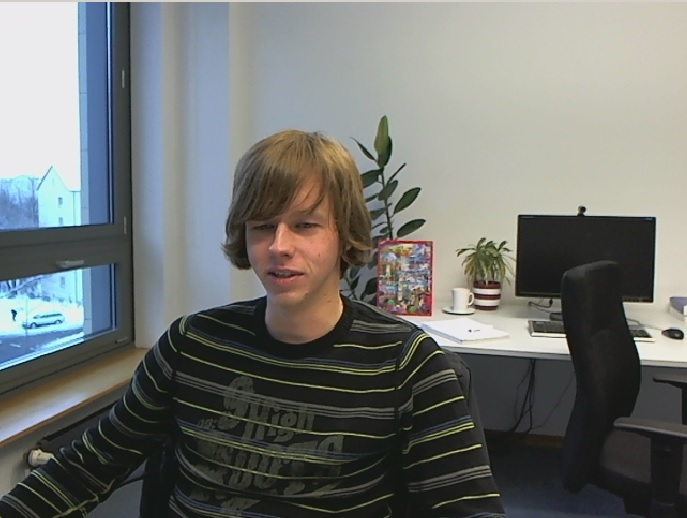
\includegraphics[scale=0.5]{PaulDefault120}
    \caption{A Frame in the input video}
    \label{fig:PaulDefault120}
%%encoded frame image
    
\includegraphics[scale=0.5]{PaulDefault120_91250kbps}
    \caption{Sample frame of fig \ref{fig:PaulDefault120} encoded at 250kbps}
    \label{fig:PaulDefaultencoded}
\end{figure} 

In a QP scale map, the darker regions in a frame indicate higher quantization. Even though quantization parameter used for encoding a block is closely related to the PSNR of the block, it is not the only determinative factor. The PSNR can also vary depending on the content. Generally, the lower frequency regions have better PSNR even when encoded with a higher QP. Also when a region of the frame is static, it tends to have better PSNR even when higher QP is used because of very less new information to be encoded. The PSNR map helps in visualizing the effect of movement of bits from non-ROI to ROI parts.

The image in Figure \ref{fig:PaulDefault120} shows a frame in the sample video conferencing content with resolution of 640x480 pixels and 30 frames per second. The image in figure \ref{fig:PaulDefaultencoded} shows the same frame when encoded with the codec configurations discussed in the previous section. The reason for considering a low bitrate of 250 kbps is that it will help in making the improvement in face region and decrease in quality of background more evident and hence will be useful in evaluating different algorithms. 

\begin{figure}[!h]
    \centering
    
\includegraphics[scale=0.5]{PaulDefault120_91250kbps_quant}
    \caption{Quantization map}
    \label{fig:PaulDefault120Quant}
    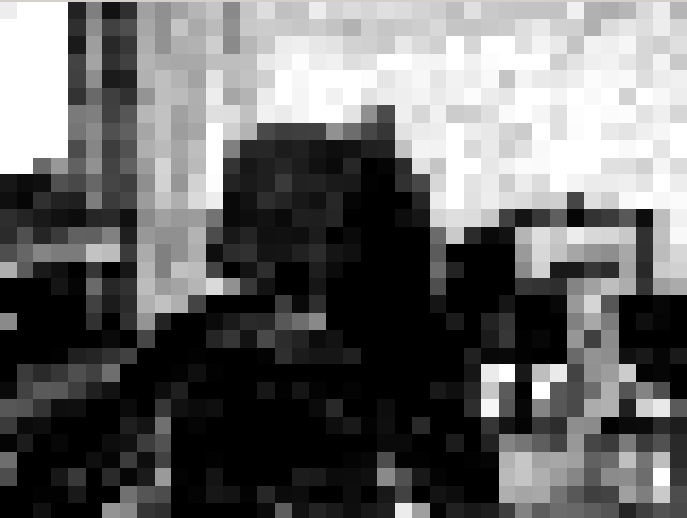
\includegraphics[scale=0.5]{PaulDefault120_91250kbps_psnr}
    \caption{Relative PSNR map}
    \label{fig:PaulDefault120PSNR}
\end{figure} 

The image in Figure \ref{fig:PaulDefault120Quant} shows the quant map of the frame in Figure \ref{fig:PaulDefaultencoded}. The darker regions in this map indicate usage of higher quantization parameter compared to the lighter regions. It can be noticed that since no information about region of interest is used while encoding the frame, the pattern of quantization appears almost random. The shape of the original content is almost not recognizable from the quantization map.

The image in Figure \ref{fig:PaulDefault120PSNR} shows the PSNR distribution for the frame in Figure \ref{fig:PaulDefaultencoded}. Similar to the quantization map, the lighter regions here represent the regions with higher PSNR, the darker regions indicate lower PSNR and worse quality. This map is relative within the frame and does not represent  absolute quality. This map is generated by considering the full range of PSNR of the image after removal of outliers. The map is generated by mapping the PSNR range between 10th percentile and 90th percentile of the whole frame to values between 0 to 255.

It is evident that the structure of the original content is preserved in the PSNR map. The background regions have better PSNR, the foreground has worse quality and the difference in quality is quite huge. The difference in the quality is due to the fact that background in a video conferencing scenario is mostly static and hence gets encoded better with every frame. On the other hand, the foreground has motion and new data to be encoded, hence it cannot achieve the same quality as the background. Since the focus of attention during video telephony is foreground or the face region, improving the face region must help in improving overall perceptual quality. The effect of such preferential encoding is studied in this work. The idea is to reduce the PSNR difference between foreground and background and to boost the quality of foreground (specifically face regions) to same level as background or even better.
%%
%%Bitrate Fluctuation and delay plots
%%
\subsubsection{Bitrate fluctuation - Delay plots} \label{sec: setup delay plots}
The core idea in this work is to efficiently use the bits within the frame to encode the region of interest. The algorithms used to achieve that purpose should not alter the behavior of the codec in terms of frame level bit-consumption. As mentioned in previous sections, the encoder drops the frame in order to maintain strict VBV buffer compliance. The dropped frames result in jerky playback and hence should be avoided. The intelligent bit-allocation scheme should not contribute to more dropped frames.

The measured delay of every frame in the sequence is plotted to analyze bit-consumption behavior. A plot the delay of each frame is used to verify this. Figure \ref{fig:PaulDefault250kbpsDelay} is the delay plot of the bitstream encoded with 250 kbps (illustrated in Figure \ref{fig:PaulDefaultencoded}). Every point in the plot specifies the time taken by the corresponding frame (marked on the x-axis) to reach the decoder assuming zero transmission delay. The curve appears mostly smooth except for sudden drops (zero values). These zero-valued points indicate dropped frames. Since these frames are not included in the final bitstream and hence not transmitted, the delay is indicated as zero. 
\begin{figure}[!h]
    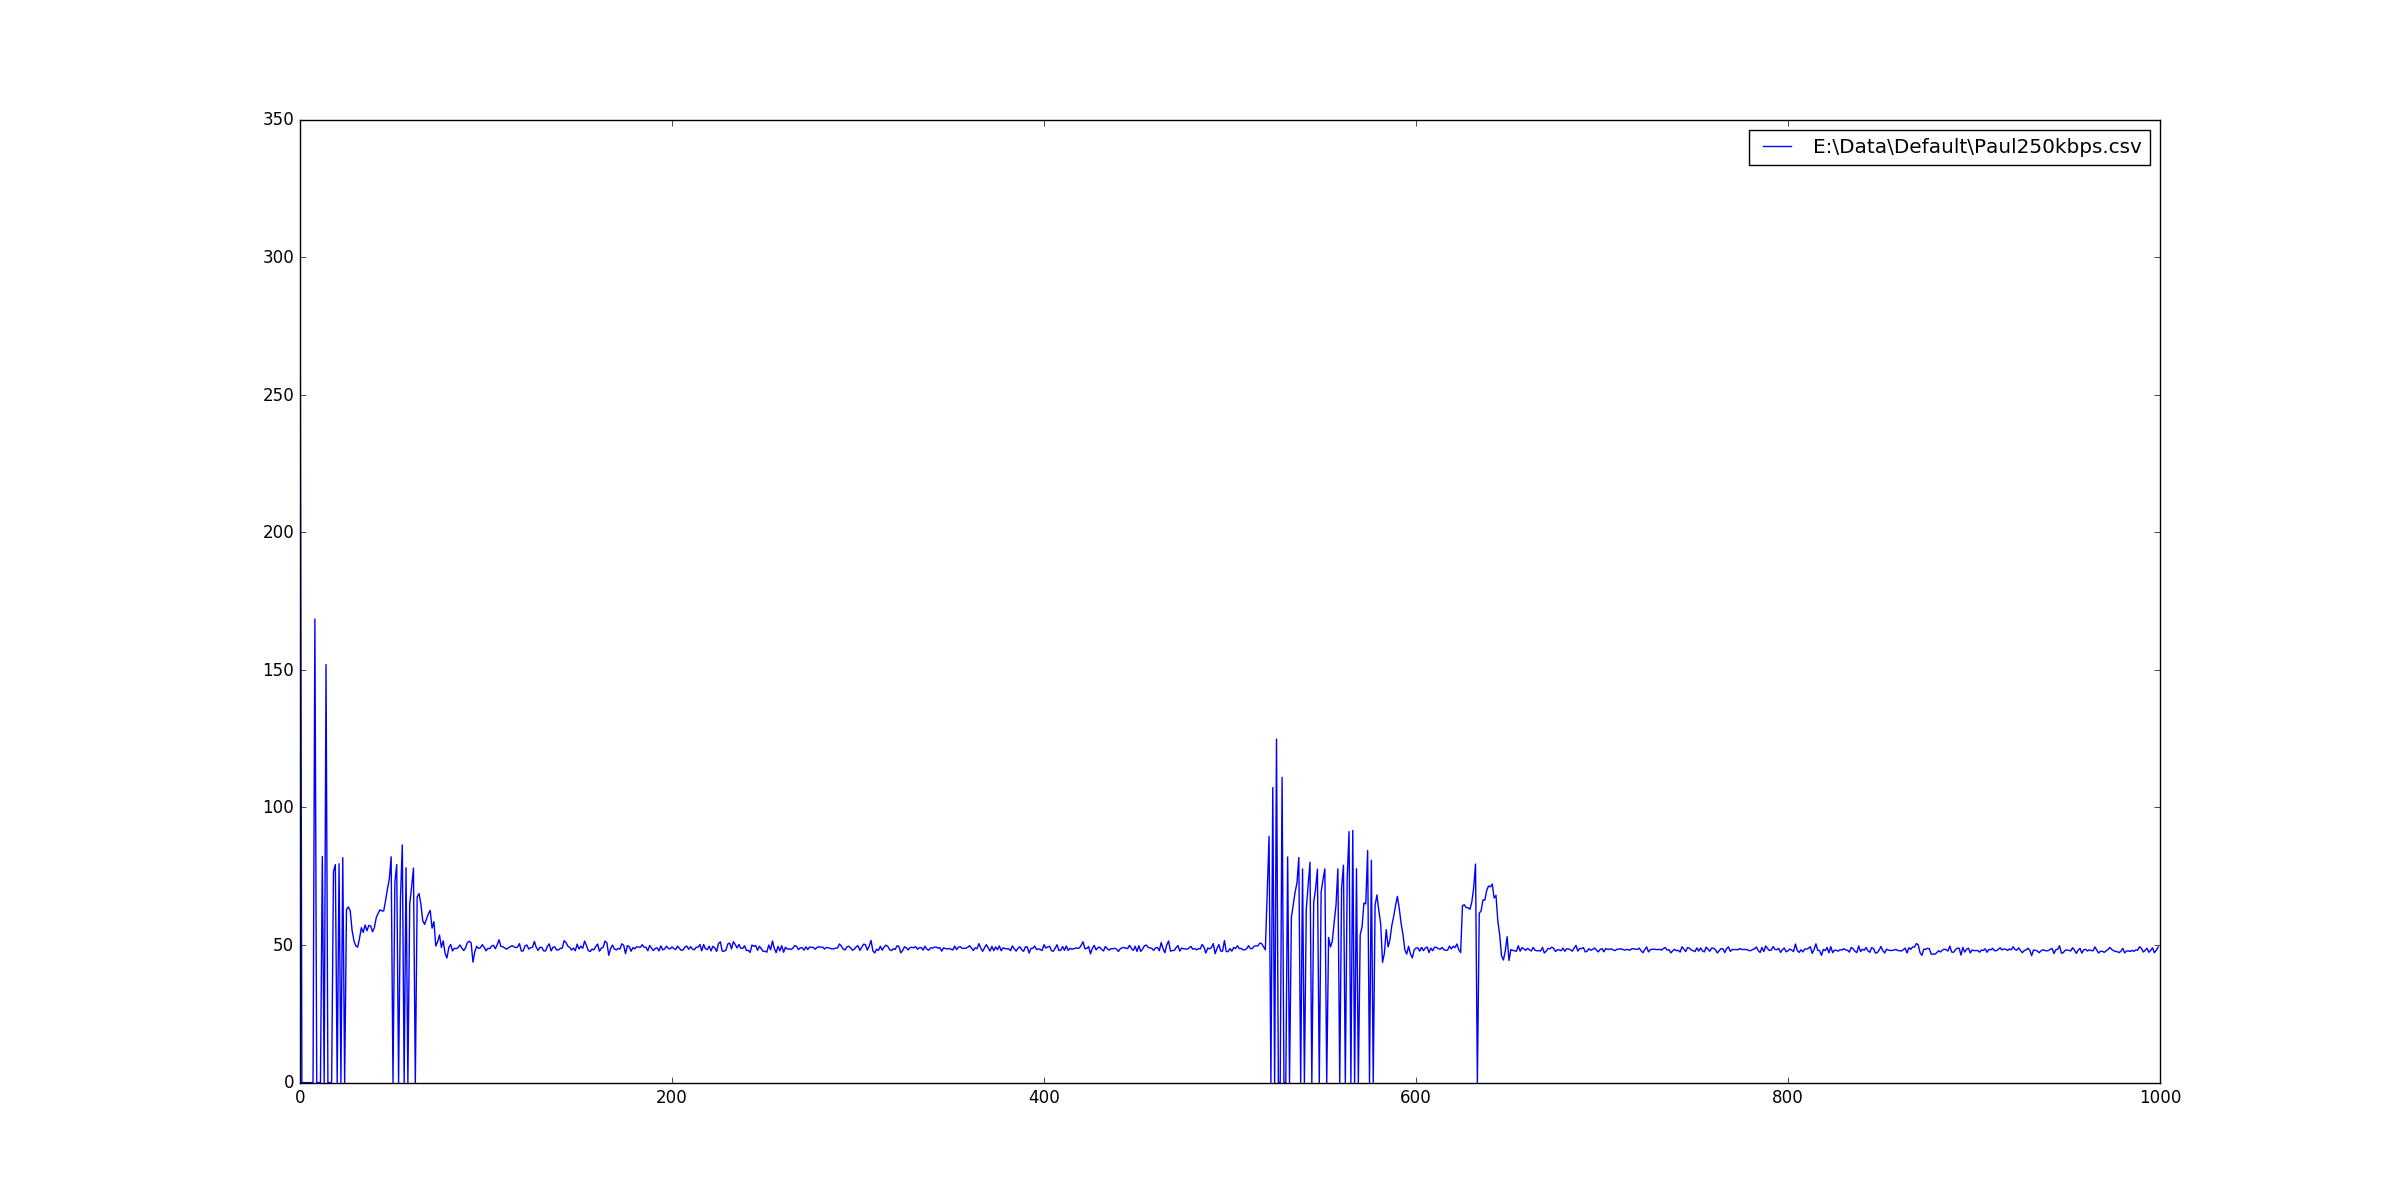
\includegraphics[scale=0.25]{PaulDefault250kbpsDelay}
    \caption{Delay plot}
    \label{fig:PaulDefault250kbpsDelay}
\end{figure} 
Ideally, an algorithm with intelligent bit allocation within a frame should not alter the shape of this graph. It is also desirable to not have any increase in the number of dropped frames. %Since, the algorithm is not expected to change overall behavior it is not expected to have reduction in number of dropped frames.
%
%Face Detection
%
\section{Face Detection}

Face detection algorithms are used to mark the region of interest in the current frame. All the algorithms considered for intelligent bit allocation involve improving the region of interest at the cost of rest of the frame. Therefore, it is very important to have high reliability with face detection. Any false detection will lead to degradation of the actual region of interest compared to normal encoding, this should be avoided in all scenarios. The damage caused by false detection is higher than the loss due to not detecting any face. Therefore, a high threshold must be used to declare any region of the frame as face.
\begin{figure}[!h]
    \centering
    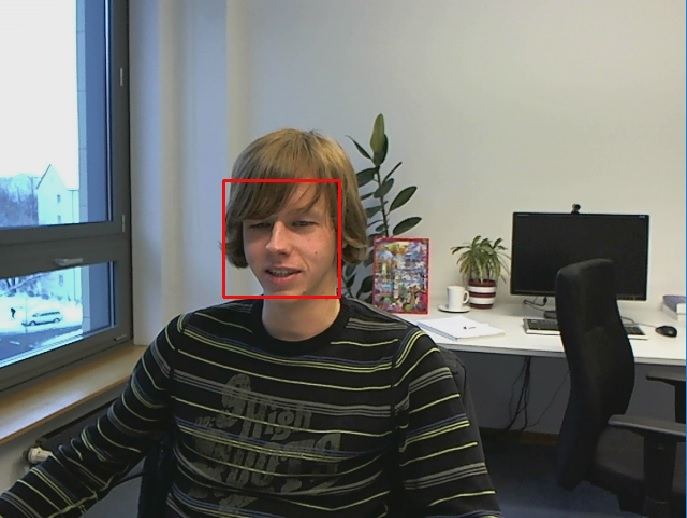
\includegraphics[scale=0.4]{PaulDefault120FaceRecognized}
    
\includegraphics[scale=0.4]{PaulDefault120FaceMap}
    \caption{Face Detection binary map}
    \label{fig:PaulDefault120FaceMap}
\end{figure}

 The face detection module itself shall not be a part of the encoder, but the output from the face detection is a binary file with face regions marked is used as input by the encoder. In this work, the face detection module uses input YUV to the encoder and marks the region of interest at the macro block level. Each byte value in the output file of face detection module represents a macro-block scanned in raster scan order. A value of 0xff signifies macro-block being part of the face or region of interest and 0x00 represents a normal macro-block. Figure \ref{fig:PaulDefault120FaceMap} represents the face map generated for the frame shown in Figure \ref{fig:PaulDefault120}. The region in white is considered as region of interest, this information is used inside the bitrate control module of the encoder to perform intelligent bit allocation.

Different approaches are used to detect the face region in the video. There is always a trade-off between accuracy of face detection algorithm and its complexity. The work presented here is mostly relevant to real time systems. Any added complexity due to additional module of face detection will cause significant delay which is totally unacceptable in such systems. Therefore, the algorithm chosen for face detection must be light weight and reasonably accurate in all lighting conditions. 

\subsection{Spatial Domain Face Detection}
In this approach, the face detection algorithms work directly on the pixel values. This approach is simple in terms of implementation. Many open-source solutions like OpenCV offers a ready to use solution that can be integrated with the codec library. It has large set of trained classifiers considering many types of faces and viewing angles. However, this is a computation intensive approach and almost impractical to use in the final solution. 
\subsection{Compressed domain Face Detection}
Most available face detection algorithms work on the pixel domain. These algorithms provide good level of detection accuracy. The main drawback of this approach is that they are computationally intensive. As discussed earlier, the use case considered in this work has very less room for additional computations. Therefore, in this work ways of compressed domain face detection is explored to detect faces with less computational requirements. 
Many works have been published
TBD LATER
%
%Different approaches
%
% 
\section{ROI-based Intelligent Bitrate Control - Approaches}
As discussed in the previous sections there are many ways in which ROI information can be used to improve the perceptual quality of the video. This section describes various approaches to modify bitrate control module to enhance the quality of ROI macroblocks. These approaches are designed considering the bitrate control module presented in section \ref{sec:used-bitrate-control-overview}. However, the underlying principles of ROI-based encoding to create the optimal quality difference between ROI and non-ROI are applicable to generic bitrate control modules to produce equivalent results. The approaches presented here vary in terms of ease of implementation, complexity and output quality. This offers flexibility to choose the suitable approach according to specific needs.

\subsection{QP offset}
The simplest way of creating a bias in the quality between ROI and non-ROI is by using a QP offset for macroblocks belonging to the ROI. A negative QP offset is added to the QP allocated by the bitrate control module (\ref{Eq:mainQP}) for ROI macroblocks. The QP offset is used outside of the bitrate control module, hence this approach requires minimum or no modifications inside the bitrate control module. The rate control module obtains feedback from the encoder regarding bit-consumption at the macroblock level (Section \ref{sec:used-bitrate-control-overview}). This feedback is used by the bitrate control module to modify the rate control QP allocation according to the externally added QP offset. The bitrate control reacts to the usage of reduced QP for ROI macroblocks by increasing the QP of non-ROI blocks to compensate for the additional bits used by ROI macroblocks. The feedback from the encoder to bitrate control module will ensure that target bitrate is successfully achieved. The bit-allocation based on buffer level (section \ref{used-bit-allocation-overview}) will ensure that a constant delay is maintained even after using the QP offset. This approach offers the simplest way of implementing quality bias without breaking the core functionality of the bitrate control module.  

\iffalse
\begin{figure}[!h]
    \centering
    
\includegraphics[scale=0.4]{PaulDefault120_91250kbps}
    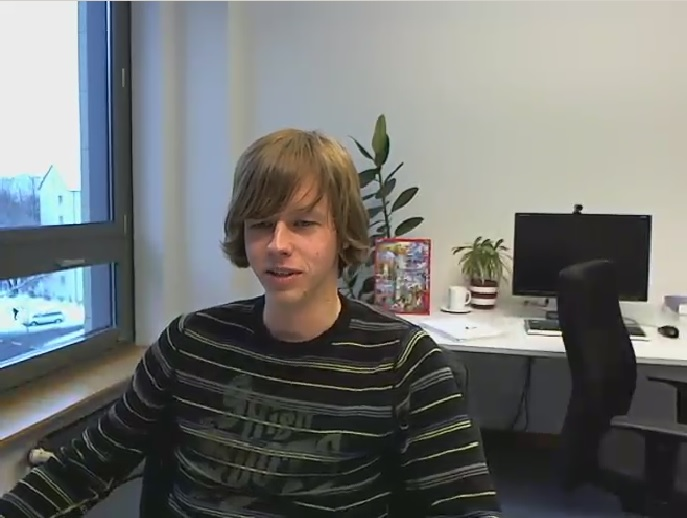
\includegraphics[scale=0.4]{QPOffset/paul120_250kbps_QPoffset4}
    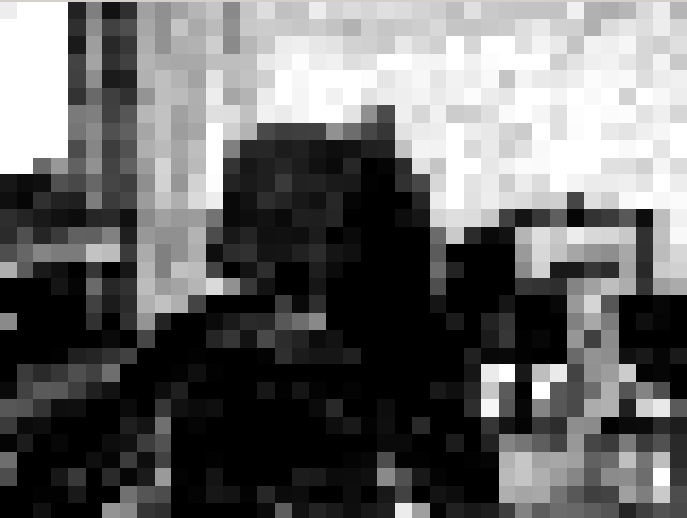
\includegraphics[scale=0.4]{PaulDefault120_91250kbps_psnr}
    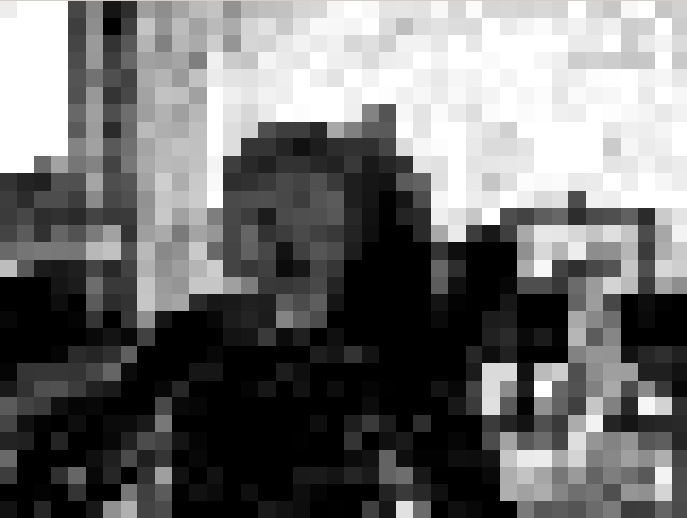
\includegraphics[scale=0.4]{QPOffset/paul120_250kbps_QPoffset4_psnr}
    
\includegraphics[scale=0.37]{PaulDefault120_91250kbps_quant}
    
\includegraphics[scale=0.4]{QPOffset/paul120_250kbps_QPoffset4_quant}    
    \caption{Comparing the images with QP offset of 4 for ROI}
    \label{fig:Default_QPOffsetCompareold}
\end{figure}
\fi

%
\begin{figure}
	\centering
	\begin{subfigure}[t]{0.45\textwidth}
		\centering
		
\includegraphics[width=\textwidth]{PaulDefault120_91250kbps}
		\caption{}
		\label{fig:QP Offset image comparison 1}
	\end{subfigure}
	\begin{subfigure}[t]{0.45\textwidth}
		\centering
		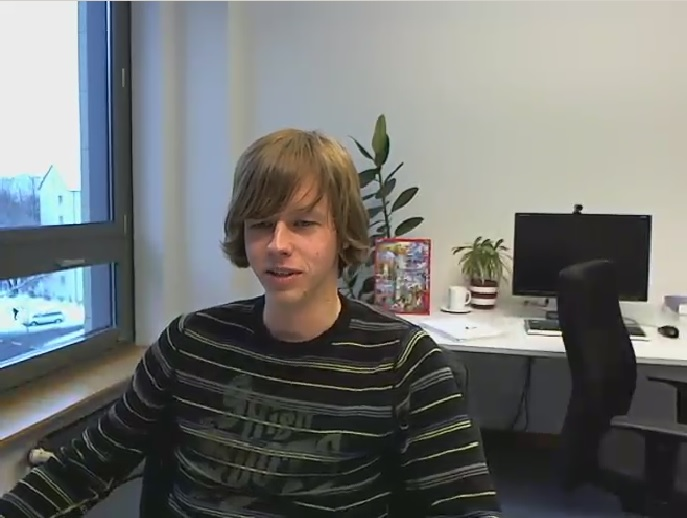
\includegraphics[width=\textwidth]{QPOffset/paul120_250kbps_QPoffset4}
		\caption{}
		\label{fig:QP Offset image comparison 2}
	\end{subfigure}
	\begin{subfigure}[t]{0.45\textwidth}
		\centering
		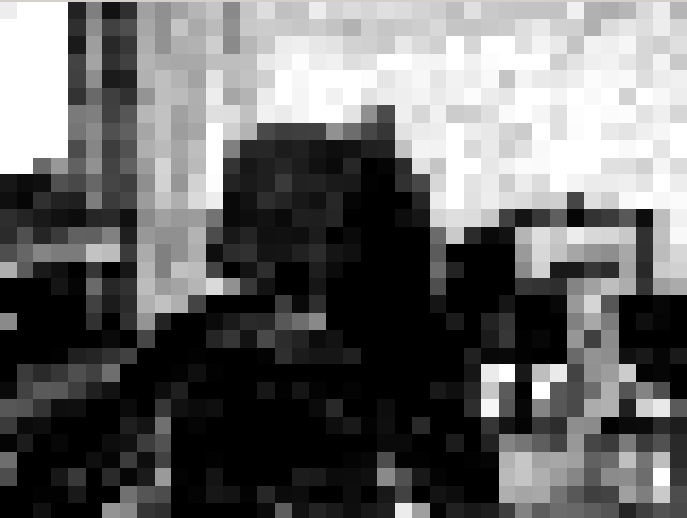
\includegraphics[width=\textwidth]{PaulDefault120_91250kbps_psnr}
		\caption{}
		\label{fig:QP Offset PSNR comparison 1}
	\end{subfigure}
	\begin{subfigure}[t]{0.45\textwidth}
		\centering
		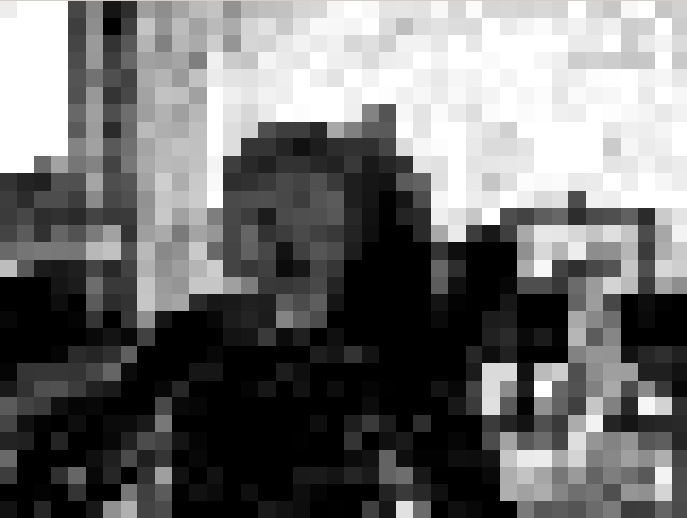
\includegraphics[width=\textwidth]{QPOffset/paul120_250kbps_QPoffset4_psnr}
		\caption{}
		\label{fig:QP Offset PSNR comparison 2}
	\end{subfigure}
	\begin{subfigure}[t]{0.45\textwidth}
		\centering
		
\includegraphics[width=\textwidth]{PaulDefault120_91250kbps_quant}
		\caption{}
	\label{fig:QP Offset Quant comparison 1}
	\end{subfigure}
	\begin{subfigure}[t]{0.45\textwidth}
		\centering
		
\includegraphics[width=\textwidth]{QPOffset/paul120_250kbps_QPoffset4_quant}
		\caption{}
		\label {fig:QP Offset Quant comparison 2}
	\end{subfigure}
	\caption{The Comparison of normal encoding vs ROI-based encoding with QP offset of 4 for ROI. The figures (a), (c), (e) and  (b), (d), (f) correspond to normal encoding and QP offset ROI-encoding approach respectively. (a) and (b) is a snapshot from the encoded output. (c) and (d) are PSNR maps and (e), (f)  are Quantization maps corresponding frames in (a) and (b).}
	\label{fig:Default_QPOffsetCompare}
\end{figure}

\begin{figure}[!h]
    \centering
    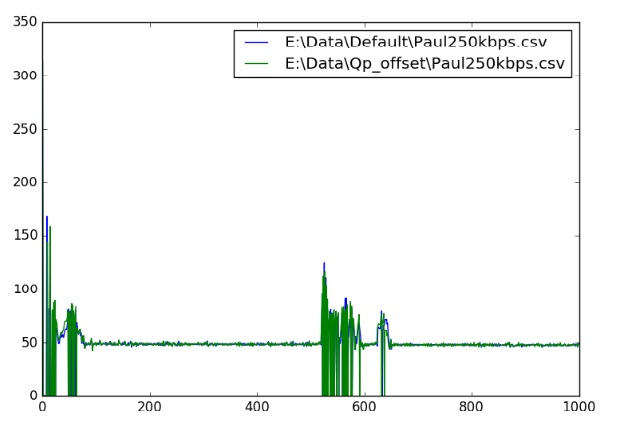
\includegraphics[scale=0.75]{QPOffset/Paul250kbps_QP_Offset_Delay}
    \caption{Delay plot of normal encoding and ROI-based encoding with QP offset of 4 for ROI}
    \label{fig:DelayDefault_QPOffsetCompare}
\end{figure}

The images in Figure \ref{fig:Default_QPOffsetCompare} shows the comparison between normal encoding and ROI-based encoding using QP offset and their corresponding attributes like PSNR map and  quantization map. The image in Figure \ref{fig:QP Offset image comparison 2} looks better in face regions compared to Figure \ref{fig:QP Offset image comparison 1} due to usage of negative QP offset for ROI. This improves the overall perceptual quality in a video. Figure \ref{fig:QP Offset Quant comparison 1}-\ref{fig:QP Offset Quant comparison 2} shows the effect of QP offset on the final QP used for encoding the macroblock. The macroblocks in the face region of \ref{fig:QP Offset Quant comparison 2} have lower QP which is seen as  macroblocks with a lighter shade of gray compared to other macroblocks in the frame. 

 The PSNR maps in Figure \ref{fig:QP Offset PSNR comparison 1}-\ref{fig:QP Offset PSNR comparison 2} shows that the PSNR of the face is closer to the background region with ROI-based encoding using QP offset. There is no major difference in the PSNR of the background region (non-ROI). The face appears much sharper due to the additional boost in quality from reduced QP. The overall bitrate of both the compared bitstreams remained almost same. The difference in the perceptual quality is only due to the movement of bits from non-ROI to ROI macroblocks. 
 
 Figure \ref{fig:DelayDefault_QPOffsetCompare} shows the delay plot described in section \ref{sec: setup delay plots} for both normal encoding and ROI-based encoding using QP offset. The visibility of single color predominantly shows that there is no significant change in bit-consumption at the frame level. This implies that the additional bits consumed by ROI macroblocks are compensated for in non-ROI blocks within a given frame. There is very less difference in bit-consumption at frame level that is carried over to the next frame. There is no significant change in number of dropped frames which is represented as zero points on the delay plot. The number of dropped frames with normal encoding and ROI-based encoding remains the same. The dropped frames also appear at the same time interval in both output bitstreams.
 
\begin{table} [h!]
\centering
\begin{tabular}{ |c|c|c|c| }
 \hline
Methodology & Content & PSNR Avg (dB) & PSNR ROI (dB) \\
 \hline 
QP Offset & Paul640x480, 250kbps & 38.90 & 38.88 \\ 
 & Johny1280x720 750kbps & 40.49 & 40.22 \\  
 \hline
Reaction Factor & Paul640x480, 250kbps & 38.22 & 39.50 \\ 
 & Johny1280x720 750kbps & 39.71 & 40.74 \\  
 \hline
ROI-based Bit-allocation & Paul640x480, 250kbps & 38.86 & 39.70 \\ 
& Johny1280x720 750kbps & - & - \\  
\hline 
\end{tabular}
 \caption{PSNR Comparison for different approaches of ROI encoding}
 \label{AllPSNR1}
\end{table}

The PSNR of ROI-based encoding with QP offset is tabulated in Table \ref{AllPSNR1}. There is a considerable improvement in the ROI PSNR. The ROI PSNR is closer to the overall frame PSNR with ROI-based encoding compared to the normal encoding results shown in Table \ref{InitPSNR1}. The boost in PSNR of the ROI is dependent on the magnitude of QP offset used for the ROI macroblocks. It is necessary to tune the QP offset to result in optimal PSNR for ROI and non-ROI to achieve improved perceptual quality. The tuning of QP offset is discussed in section \ref{sec:Tuning QP Offset}.


\iffalse
which However, this approach might result in bitrate control over-reacting for the blocks around the ROI and encode them with extremely low quality. The magnitude of QP offset shall dictate the magnitude of shift in quality for the ROI. This approach is used to find right QP offset for best perceptual quality.\\

It is perhaps a better idea to link the confidence quotient of face detection algorithms with the QP offset used. It should also be dependent on the area of the face, if the area of the ROI is considerably large in a video then the quality difference should be minimized. This is because there will be less non-ROI regions to compensate for additional bits used in ROI.
\fi

%
\subsubsection{Tuning QP Offset} \label{sec:Tuning QP Offset}
As mentioned earlier, the methods discussed in this work only aim to re-distribute the bits within a frame based on the region of interest. The magnitude of re-distribution should be carefully chosen to avoid degradation of the background to an extent that artifacts become noticeable to the viewer even though they are not expected to concentrate on those regions. The ideal level of redistribution will make sure that there is a maximum transfer of bits from non-ROI part to ROI part without creating any visible artifacts in the image.
\iffalse
\begin{figure}[!h]
    \centering
    
\includegraphics[scale=0.43]{QPOffset/trialOffset/Paul250kbps_offset2}
    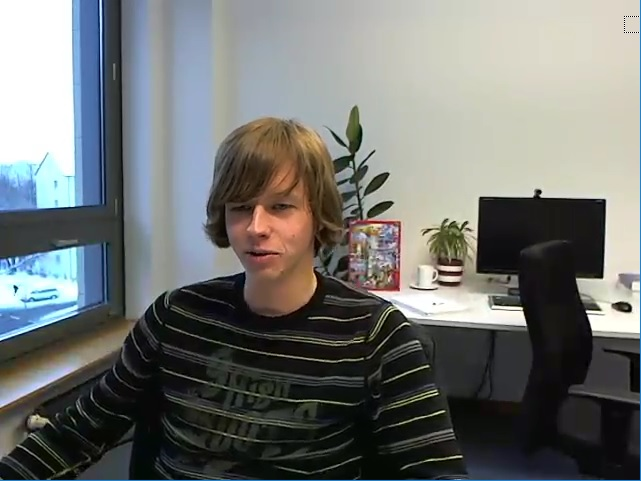
\includegraphics[scale=0.43]{QPOffset/trialOffset/Paul250kbps_offset4}
    
\includegraphics[scale=0.43]{QPOffset/trialOffset/Paul250kbps_offset6}
    
\includegraphics[scale=0.43]{QPOffset/trialOffset/Paul250kbps_offset8}  
    \caption{Tuning QP offset - Trial QP offsets used are 2, 4, 6 and 8 in raster scan order}
    \label{fig:Default_QPOffsetTuning}
\end{figure}
\fi


%
\begin{figure}
	\centering
	\begin{subfigure}[t]{\textwidth}
		\centering
		
\includegraphics[width=0.49\textwidth]{Tuning_QP_offset/QP_offset_8/with_swing_restriction/Paul250kbps_uni_QP_offset_8.jpg}
		
\includegraphics[width=0.49\textwidth]{Tuning_QP_offset/QP_offset_8/with_swing_restriction/Paul250kbps_uni_QP_offset_8_psnr_abs.jpg}
		\caption{QP offset = -8}
		\label{fig:QP offset compare 8}
	\end{subfigure}
	\begin{subfigure}[t]{\textwidth}
		\centering
		
\includegraphics[width=0.49\textwidth]{Tuning_QP_offset/QP_offset_12/with_swing_restriction/Paul250kbps_uni_QP_offset_12.jpg}
		
\includegraphics[width=0.49\textwidth]{Tuning_QP_offset/QP_offset_12/with_swing_restriction/Paul250kbps_uni_QP_offset_12_psnr_abs.jpg}
		\caption{QP offset = -12}
		\label{fig:QP offset compare 12}
	\end{subfigure}
	\caption{The snapshot of ROI-encoded test sequence (Left) and its corresponding absolute PSNR map (Right) for different QP offset.}
	\label{fig:QP offset tuning}
\end{figure}


%Table to show number of dropped frames
\begin{table} [h!]
	\centering
	\begin{tabular}{ |c|c|c| }
		\hline
		\textbf{ROI QP Offset} & \textbf{Swing Restriction = on} & \textbf{Swing Restriction = off} \\
		\hline 
		0 & 16 & 10  \\
		\hline
		-4 & 19 & 11  \\
		\hline
		-8 & 31 & 11 \\ 
		\hline
		-12 & 45 & 11 \\ 
		\hline						
	\end{tabular}
	\caption{Number of dropped frames with different QP offsets for ROI for test sequence with 1000 frames.}
	\label{Table:QP tuning dropped frames}
\end{table}

In this work, various offsets were used to study the effect of the magnitude of QP offset on perceptual quality. The results of ROI-based encoding with QP offset of -4 shows favorable results with increased perceptual quality. This section examines the impact of increasing the magnitude of QP offset further. %The results shown in Figure \ref{fig:QP offset tuning} shows that, as QP offset increases the face region appears more sharper which improves the overall perceptual quality of the frame. 

The snapshot of sample input encoded  with QP offset of -8 shown in Figure \ref{fig:QP offset compare 8} appears to not have any noticeable blockiness in the background. However, with further increase in the magnitude of QP offset the blockiness in the background becomes more prominent. The image in Figure \ref{fig:QP offset compare 12} is encoded with QP offset of -12. Due to the QP swing restriction discussed in section \ref{sec: Bitrate overview: Bitrate deviation}, the difference in QP across macroblocks is heavily restricted. The maximum value of macroblock QP ($QP_{max}$) given by (\ref{Eq:QP swing restriction}), avoids the excessive degradation of the non-ROI macroblocks due to the usage of large QP offset. The QP of non-ROI blocks is not allowed to go very high despite over-consumption of bits by ROI blocks.  The side-effects of increased QP offset shows up in the form of an increase in the number of dropped frames. Table \ref{Table:QP tuning dropped frames} shows the number of dropped frames in the encoded video with 1000 input frames. There is a drastic increase in the number of dropped frames with QP offset of -8 and -12. This increase in dropped frames reduces the smoothness of the playback which is annoying to the viewer.

When the QP swing restriction was turned off temporarily, the number of dropped frames with increased QP offset reduced drastically as shown in Table \ref{Table:QP tuning dropped frames}. There was no considerable increase in dropped frames compared to the output of normal encoding without using any ROI information. However, the quality of non-ROI blocks dropped significantly without QP swing restrictions. The extreme blockiness in the non-ROI regions decreased the perceptual quality. Therefore, using large QP offsets can lead to less perceptual quality either due to increased dropped frames or excessive blockiness in the background depending on the configuration of QP swing restriction. Therefore, the QP offset for the ROI should be tuned not only considering the degradation of the background quality but also by assessing any other side-effects like an increase in the number of dropped frames.

%
%Discuss the impact of ratio of ROI mbs to non-ROI mb's
\subsubsection{Area of Region of Interest}
This section discusses the importance of considering the relative area of ROI with respect to non-ROI parts in calculating the QP offsets. The variation in QP offset discussed in the above section corresponds to the sample input content which has a similar ratio of number of ROI macroblocks to number of non-ROI macroblocks across all the frames. In the sample sequence used, 46 to 50 macroblocks out of a total of 1200 macroblocks belong to the face region(ROI) in each frame. Therefore, the ROI is less than 5 percent of the entire video frame. Due to the small percentage of ROI blocks, it is possible to use large QP offset (very low ROI QP) since there are a large number of non-ROI macroblocks to compensate for the over-consumption of bits by ROI macroblocks. However, in a video conferencing scenario,  based on the focal length of the camera and distance of the participant from the camera, area of the face in the video frame can change significantly. The number of ROI macroblocks can also change within a given input content. This requires continuous adaptation of QP offset to avoid visual artifacts due to the usage of wrong QP offset. For instance, when the area of ROI is half of the entire frame, usage of higher QP offsets will cause severe degradation in the quality of non-ROI macroblocks. In order to avoid severe degradation of the background, the magnitude of the QP offset should be inversely proportional to the ratio of the number of ROI blocks to the number of non-ROI blocks.

The algorithm implemented to adapt QP offset uses relative area of ROI. The QP offset is calculated using linear relationship described in (\ref{Eq:QP_offset}). The scaled QP offset is then clipped to a value of -6 to avoid large QP offsets which can lead to side-effects discussed in the above section.
\begin{equation}
	\label{Eq:QP_offset}
	\begin{aligned}
	dq_{roi'} = -round\Big(\frac{M}{M_{roi} * 3}\Big) \\
	dq_{roi} = clip(dq_{roi'}, -1 , -6)
	\end{aligned}	
\end{equation}
where, $dq_{roi}$ is the offset used for ROI blocks, $M$ is the total number of macroblocks in the frame and $M_{roi}$ is the total number of macroblocks marked as region-of-interest. The negative sign in the equation implies that the calculated offset is negative, which results is QP lower than non-ROI blocks. It is also evident from (\ref{Eq:QP_offset}) that there is no QP offset for ROI region if the ROI covers more than two-third of the whole frame. The QP offset increases linearly with subsequent decrease in the ROI area.

\subsubsection{Bi-direction QP-offset}
The QP offsets calculated so far is only applied to the ROI macroblocks. The bitrate control module is held responsible for compensating the additional bits used in encoding the ROI blocks by increasing the QP of non-ROI blocks. 

As explained in section \ref{sec: Bitrate overview: Bitrate deviation}, the bitrate control uses feedback from the encoder to constantly react to any deviation in the bitrate at the macroblock level. This feedback loop is not aware of the QP offset which is applied externally to QP computed by bitrate control. Due to this, the bitrate control reacts to over-consumption of bits by increasing the QP of non-ROI blocks only after encoding the ROI macroblocks. This effect can is clearly seen in the quant map of ROI-based encoding in Figure \ref{fig:QP Offset Quant comparison 2}. The macroblocks encoded immediately after ROI have larger QP (depicted as a darker shade of gray). Therefore, this approach does not increase the QP of non-ROI blocks uniformly. The non-ROI blocks encoded before ROI blocks have no increase in QP since reaction by rate control to increased deviation in bitrate is not triggered until the ROI macroblocks are encoded. The non-ROI macroblocks encoded after ROI blocks tend to have lesser quality than the non-ROI blocks encoded before the ROI blocks. This non-uniform loss of quality in non-ROI blocks is not desirable for good perceptual quality.

The non-uniform increase in non-ROI QP also depends on the position of the ROI within the video frame. For instance, consider a content where the ROI part in the frame falls in the bottom right corner of the frame. Assuming that macroblocks are encoded in the raster-scan order, the over-consumption of bits by the ROI part cannot be compensated within that frame. The error is carried over to the next frame. This alters the frame level bit-consumption behavior and can lead to increased number of dropped frames in extreme cases. 

A Bi-direction QP offset is used to avoid the behavior described above. The non-ROI blocks are assigned with positive QP offset, which can compensate the over-consumption in ROI blocks. The non-ROI blocks are encoded with a higher QP even before ROI blocks are encoded. Since the non-ROI blocks from the start of the frame are encoded with higher QP, there will be a surplus of bits already which can be used in encoding ROI blocks. In an ideal scenario, the negative and positive QP offsets must negate each other's effect resulting in frame level bits being unchanged had the frame been encoded without any offset.

The study in \cite{ROI-Coding-paper} suggests that for the frame level bitcount to be constant, the average QP of the frame must remain unchanged before and after adding the offsets. This is an observation made after multiple experiments. The QP offset for non-ROI macroblocks used to compensate for negative QP offset used by ROI is given by,
\begin{equation}
	\label{Eq:QP_offset_double}
		dq_{nroi} = \frac{M_{roi} * dq_{roi}}{M - M_{roi}}
\end{equation}
where, $dq_{nroi}$ is a positive QP offset used for non-ROI blocks when negative QP offset of $dq_{roi}$ is used for ROI blocks (\ref{Eq:QP_offset}). 

%%Results of Two-sided QP offset
\begin{figure}
	\centering
	\begin{subfigure}[t]{0.49\textwidth}
		\centering
		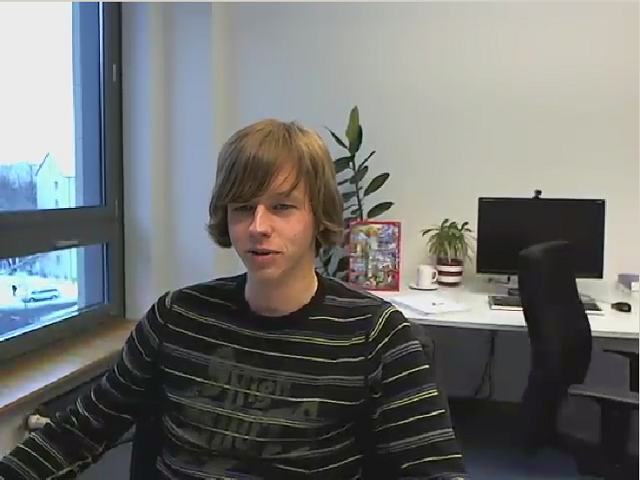
\includegraphics[width=\textwidth]{QPOffset/Bi_direction/Paul250kbps_uni_QP_offset_Bi_4.png}
		\caption{}
		\label{fig:Bi-direction QP offset result image}
	\end{subfigure}
	\begin{subfigure}[t]{0.49\textwidth}
		\centering
		
\includegraphics[width=\textwidth]{QPOffset/Bi_direction/Paul250kbps_uni_QP_offset_Bi_4_psnr_abs.png}
		\caption{}
		\label{fig:Bi-direction QP offset result psnr}
	\end{subfigure}
	\begin{subfigure}[t]{\textwidth}
	\centering
	
\includegraphics[width=0.49\textwidth]{QPOffset/Bi_direction/Paul250kbps_uni_QP_offset_Bi_4_quant.png}
	\caption{}
	\label{fig:Bi-direction QP offset result quant}
	\end{subfigure}
	\caption{The results of ROI-based encoding with Bi-direction QP offset.(a) Snapshot of encoded video, (b) absolute PSNR map (range 25dB - 50dB), (c) quantization map}
	\label{fig:Bi-direction QP offset result}
\end{figure}

\subsubsection{Results}
The results of improved QP offset based ROI encoding is shown in Figure \ref{fig:Bi-direction QP offset result}. The improvements include using of relative area based QP offset and Bi-direction QP offset discussed in the previous sections. The quantization map shown in Figure \ref{fig:Bi-direction QP offset result quant} has less increase in the non-ROI QP compared to approach without bi-direction QP offset shown in Figure \ref{fig:QP Offset Quant comparison 2}. This approach also works with any size of ROI since the QP offsets are scaled according to the relative area of the ROI.
 
This section analyses the advantages and disadvantages of ROI-based encoding using QP offsets. Since the QP offset is applied outside the bitrate control, there is less possibility of other factors like buffer fullness and global deviation ($D_m^{n'}$) overriding the QP offset. Such guaranteed QP offsets will ensure boost in the ROI quality at all circumstances. However, this approach has many side effects due to the forced QP offset. The main disadvantage of this approach is not considering the content to decide the QP offset. Any given input with a given ratio of the number of ROI blocks to the number of non-ROI blocks will have the same QP offsets irrespective of the content. The QP offset computation is empirical which might work for most of the contents. However, it is not guaranteed to give optimal results for all contents.

The advantages and disadvantages of this approach can be summarized as follows,
\subsubsection*{Advantages}
\begin{itemize}
	\item Easy to implement with minimal changes required to the encoder.
	\item QP offset is forced irrespective of buffer conditions, therefore guarantees quality difference between ROI and non-ROI.
\end{itemize}

\subsubsection*{Disadvantages}
\begin{itemize}
	\item Since buffer conditions are not considered at macroblock level, there is increased possibility of dropped frames.
%%	\item The reaction of the bitrate control to external offset is not uniform throughout the non-ROI macroblocks. The reaction is less before encoding the ROI and very high just after encoding the non-ROI. This causes non uniform quality within the non-ROI macroblocks. 
	\item The QP offsets chosen does not take into account any of the input content characteristics. Same QP offset is used for all the contents for a given ROI to non-ROI ratio.
	\item The deviation control mechanism described in section \ref{sec: Bitrate overview: Bitrate deviation} is not in sync with QP offsets. 
\end{itemize}

The next section introduces an alternative approach for ROI-based encoding using region based bit-allocation. Some of the disadvantages of the QP offset approach are addressed in the new approach.

%%Add new section for splitting bit-allocation
\subsection{ROI based Bit-Allocation}
This section introduces an approach with modifications to the bit allocation module for improved ROI-based encoding. The main drawback of the QP offset based approach is that the input video content characteristics are not considered for determining the QP offset. The difference in complexity of ROI and non-ROI macroblocks determines the magnitude of quality difference required for good perceptual quality. This magnitude of optimal quality difference varies across different contents according to variation in complexity within a frame. For instance, consider a sample input video with moving background regions (non-ROI) but a simple static foreground (ROI). The usage of heuristic QP offsets which assumes background to be mostly static will result in annoying blocky artifacts in the background. This might decrease the perceptual quality to a level below that of the video without ROI-based encoding. Therefore it is important to consider the relative complexities of ROI and non-ROI parts to compute the desired quality difference between these regions.

In this approach, the bits allocated at frame level $(B_{alloc})$ is split between the ROI and non-ROI parts based on the relative complexity of these regions. The cost of a macroblock computed during rate-distortion optimization (\ref{Eq:CostCalc}) is accumulated for ROI and non-ROI regions to get a relative complexity metric ($C_r$),
$$C_r = \frac{\sum_{i =0}^{M_{roi}}{J_i}}{\sum_{i =0}^{M-M_{roi}}{J_i}},$$
where, $j_i$ is the RDO cost of the macroblock $i$. The cost of a region determines the bits consumed by the corresponding region. The relative bit consumption of ROI and non-ROI is predicted assuming that,
\begin{equation}
\label{Eq:Relative bit consumption}
	C_r \propto B_R.
\end{equation}
where, $$B_R = \frac{B_{roi}}{B_{nroi}}.$$
Here $B_{roi}$ and $B_{nroi}$ is the accumulated bit consumption of all $M_{roi}$ macroblocks belonging to ROI and  $M_{nroi}$ non-ROI macroblocks respectively. The above equations hold true for any two regions in a given frame given that these two regions are encoded with equal importance (no ROI-encoding). Therefore, $B_{roi}$ and $B_{nroi}$ corresponds to bit consumption of the two regions if the frame was encoded normally without using any ROI information. The idea is to predict the bit-consumption in normal encoding without ROI information and allocate bits for ROI and non-ROI regions according to the estimate but with a bias for ROI part. 
 
The ROI-based encoding with modified bit-allocation involves following major steps.
\begin{itemize}
	\item Predict relative bit-consumption of ROI and non-ROI ($B_R$) without any ROI-based encoding.
	\item Split allocated frame level bits ($B_{alloc}$) between ROI and non-ROI parts according to ($B_R$) with an additional bias for ROI parts.
	\item Bitrate control for ROI and non-ROI regions.
\end{itemize}
The following sections discuss each of the above steps in detail.

\subsubsection{Relative Bit-consumption Prediction} \label{sec:Relative Bit-consumption Prediction}
The first step in bit-allocation based ROI-encoding is to determine the relative bit-consumption of the ROI and non-ROI parts ($B_R$) if the frame was encoded normally without any bias for ROI regions. In this work, the relationship between the complexity of a macroblock and its bit-consumption during normal encoding without using any ROI information is studied. The RDO cost (\ref{Eq:CostCalc}) is chosen as the complexity metric for prediction of $B_R$. The computation of a new complexity metric for predicting bit-consumption is not desirable due to increased complexity. The RDO cost which is computed by the encoder during rate-distortion optimization stage is reused to predict $B_R$. 

The RDO cost is also used in the bitrate control for delta QP prediction as discussed in section \ref{used QP prediction overview}. The cost of a macroblock affects its bit-consumption in two opposite ways. The cost of a macroblock reflects the complexity of the macroblock. A macroblock with a higher cost consumes more bits (\ref{Eq:Relative bit consumption}). On the other hand, the delta QP computation (\ref{Eq:deltaQP}) allocates a higher QP to the macroblock with a higher cost to equalize the bit-consumption across all the macroblocks. These conflicting influence of cost on bit-consumption makes it's prediction more complex. 

In the first iteration, constant QP across all the macroblocks in a frame is used for coarse prediction of relative bit-consumption from the RDO-cost. The effect of delta QP is factored in to make prediction more accurate in the later stage (TBD).

\begin{figure}[!h]
	\centering
	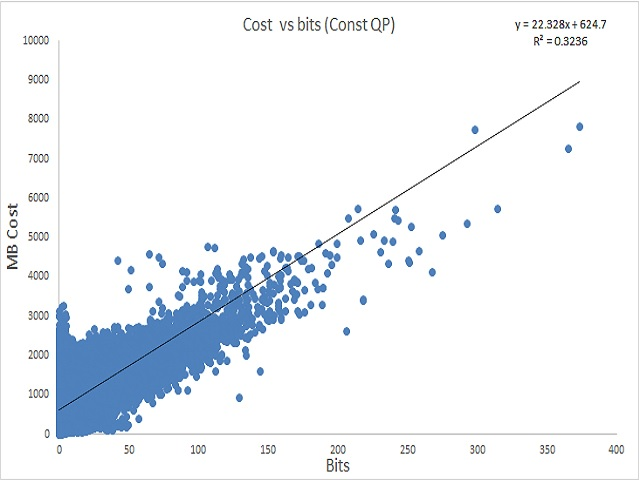
\includegraphics[scale=0.75]{CostVsBits/const_QP/CostvsBits_ConstQP_Full}  
	\caption{Macroblocks Cost vs Bits plot for all the macroblocks in a sample constant QP encoded video with 100 frames}
	\label{fig:CostvsBits_ConstQP_Full}
\end{figure}

Figure \ref{fig:CostvsBits_ConstQP_Full} shows the plot of cost vs bits at the macroblock level. Every point on this plot corresponds to bit-consumption of a macroblock and its corresponding RDO cost computed during the RDO stage. The plot corresponds to all the macroblocks in the encoded video sequence with 100 frames. The encoding for this plot was done in constant QP mode with QP=35 for all the macroblocks. The data of the first key frame is not included in this plot since the first key frame is encoded normally without using ROI information. It can be noticed that there is a linear relationship between predicted macroblock cost and the corresponding bit-consumption. 

The linear relationship between cost of a macroblock (J) and its corresponding bit-consumption (b) at a constant QP is given by,
\begin{equation}
	\label{Eq:costvsbits model all}
	J = 22.328 . b + 624.7.
\end{equation}
The above equation is obtained by performing linear regression on the entire data set shown in Figure \ref{fig:CostvsBits_ConstQP_Full}. It has a corresponding $R^2$ value of 0.3236. The $R^2$ value (also displayed on the plots) is a measure of correlation between actual data and the predicted data using the linear relationship. A value of $R^2 = 1$ indicates perfect correlation. 

The data in Figure \ref{fig:CostvsBits_ConstQP_Full} includes data for macroblocks of all types of prediction modes like skip, intra and inter prediction. It was observed that the predictability of bit-consumption using RDO cost was heavily dependent on the prediction mode used for encoding the macroblock. 

%Table to encoding mode specific data
\begin{table} [h!]
	\centering
	\begin{tabular}{ |c|c|c| }
		\hline
		\textbf{Prediction Mode} & \textbf{Occurrence Probability } & \textbf{$R^2$ value} \\
		\hline 
		Intra & 0.233 & 0.8757  \\
		\hline
		Inter & 0.28 & 0.2995  \\
		\hline
		Skip &  0.69 & 0.0412 \\ 
		\hline					
	\end{tabular}
	\caption{The probability of prediction modes in 100 frames of encoded video in constant QP (QP = 35) and its corresponding $R^2$ value.}
	\label{Table:Mode Specific data}
\end{table}

The analysis of the macroblock cost and its corresponding bit-consumption specific to encoding mode is shown in Figure \ref{fig: Cost vs bits mode}. The plots in Figure \ref{fig: Cost vs bits mode} uses the same data as shown in Figure \ref{fig:CostvsBits_ConstQP_Full} but filtered based on the mode of encoding. It can be noticed that the correlation between cost and bits is maximum for intra-prediction ($R^2 = 0.8757$) followed by inter-prediction ($R^2 = 0.2995$). However, the bit-consumption pattern was found to be almost independent of the cost for skip-mode macroblocks ($R^2 = 0.0412$). This is because skip-mode decision happens in a later stage of encoding when there are no transform coefficients generated for a macroblock encoded with intra or inter-prediction. The cost associated with skip macroblock corresponds to the encoding mode chosen before the macroblock was decided to be encoded as skip macroblock.


%Complexity vs bits prediction analysis
%%Results of Two-sided QP offset
\begin{figure}
	\centering
	\begin{subfigure}[t]{0.49\textwidth}
		\centering
		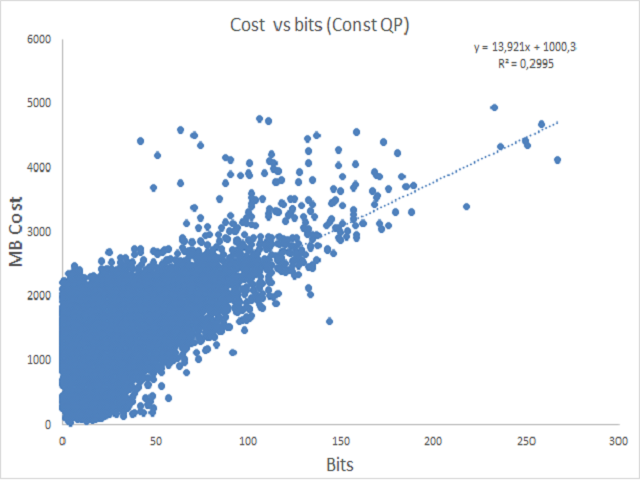
\includegraphics[width=\textwidth]{CostVsBits/const_QP/CostvsBits_ConstQP_inter.png}
		\caption{Inter Prediction mode}
		\label{fig: Cost vs bits mode inter}
	\end{subfigure}
	\begin{subfigure}[t]{0.49\textwidth}
		\centering
		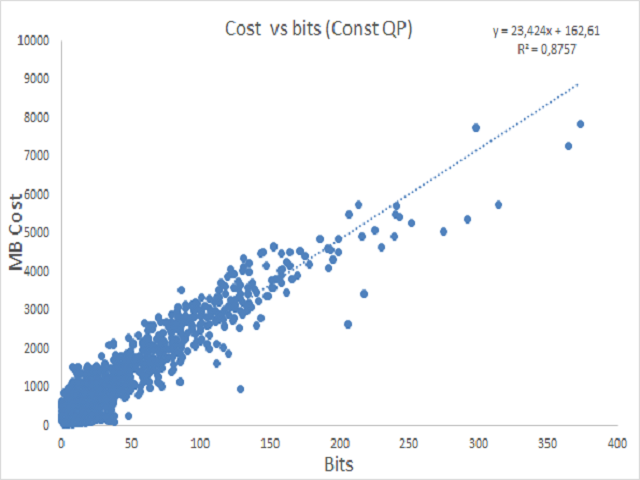
\includegraphics[width=\textwidth]{CostVsBits/const_QP/CostvsBits_ConstQP_intra.png}
		\caption{Intra Prediction mode}
		\label{fig: Cost vs bits mode intra}
	\end{subfigure}
	\begin{subfigure}[t]{\textwidth}
		\centering
		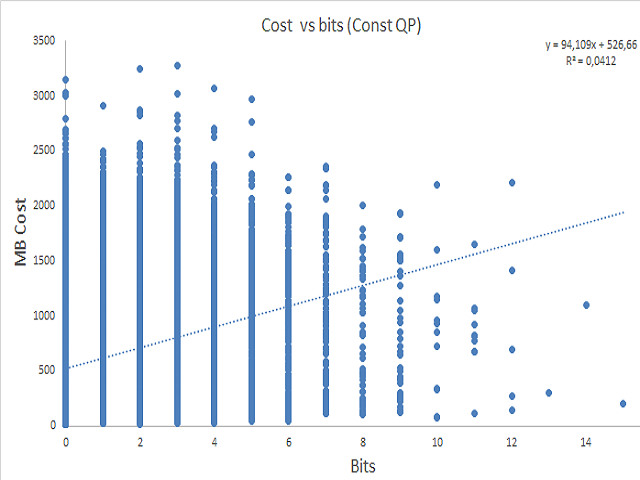
\includegraphics[width=0.49\textwidth]{CostVsBits/const_QP/CostvsBits_ConstQP_skip.png}
		\caption{Skip mode}
		\label{fig: Cost vs bits mode skip}
	\end{subfigure}
	\caption{The Cost vs Bits plots of macroblocks specific to mode of encoding. (a) inter prediction mode, (b) intra prediction mode, (c) skip mode}
	\label{fig: Cost vs bits mode}
\end{figure}
 
The uncorrelated cost and bits value can lead to large inaccuracy in predicting relative bit-consumption ($B_R$) of ROI and non-ROI parts. The data in Table \ref{Table:Mode Specific data} shows that skip mode in the most common prediction mode for the encoder configuration discussed in section \ref{sec:Encoder configuration}. This is due to low target bitrate and mostly static background in the chosen content. Therefore, it is very important to have good bits vs cost prediction model for skip macroblocks to compute $B_R$ with reasonable accuracy.

Fortunately, the uncorrelated cost and bits value for skip mode can be easily handled by assuming a constant number of bits for skip mode and ignoring its cost. The average of bits consumed by skip macroblocks over 100 frame video was found to be 0.458 bits. This value can be used directly in (\ref{Eq:Relative bit consumption}) to compute relative bit-consumption of ROI and non-ROI based on the number of skip macroblocks in each of these regions.

The steps involved in computing relative bit-consumption of ROI and non-ROI region ($B_R$) are,
\begin{itemize}
	\item Identify the ROI and non-ROI macroblocks in the input frame.
	\item Get the number of intra macroblocks, inter-macroblocks and skip macroblocks in the ROI and non-ROI region separately. This can be done using the previous frame data.
	\item Compute relative complexity of the ROI and non-ROI parts by accumulating costs of macroblocks in these regions.
	\item The relative complexity metric is translated to relative bit-consumption ($B_R$) between ROI and non-ROI using  prediction models shown in Figure \ref{fig: Cost vs bits mode}. A pre-computed value is used for skip macroblocks to account for bit consumed by skip macroblocks.
\end{itemize}

The procedure involved in using ($B_R$) to allocate bits to ROI and non-ROI parts with a bias for ROI parts to perform ROI-based encoding is discussed in subsequent sections.

\subsubsection{ROI and non-ROI Bit Allocation}
This section gives an overview of the process involved in splitting the frame level allocated bits ($B_{alloc}$) computed in (\ref{Eq:bit-allocation}) between ROI and non-ROI regions. This is done using relative bit-consumption factor ($B_R$) computed in the previous section. In the case of normal encoding without ROI information, $B_{alloc}$ is split between ROI and non-ROI according to $B_R$ (by definition of $B_R$). For ROI-based encoding, a bias factor k is introduced to create bias in bit-allocation. The bits allocated for ROI region ($B_{alloc}^{roi}$) is given by,
\begin{equation}
\label{Eq:ROI allocated bits}
B_{alloc}^{roi} = k \times B_R \times B_{alloc}^{nroi}
\end{equation}
and,
$$ B_{alloc}^{nroi} = B_{alloc} - B_{alloc}^{roi}$$
Here k is the ROI bias factor. For normal encoding without ROI information, $k = 1$. For ROI-based encoding, a value $k > 1$ is used to bias bit-allocation to allocate more bits to ROI considering its importance to the perceptual quality. The bias factor($k$) gives the flexibility of tuning the bias for ROI based on the importance of the ROI.

As mentioned earlier, the bit-allocation based ROI encoding is independent of the procedure involved in determining the relative bit-consumption factor ($B_R$). The approach presented in section \ref{sec:Relative Bit-consumption Prediction} needs computation of relative complexities of ROI and non-ROI regions. A simpler approach is to assume that the frame is uniformly complex and splitting the frame level allocated bits ($B_{alloc}$) uniformly between ROI and non-ROI with bias factor specified in (\ref{Eq:ROI allocated bits}). Therefore, if the content information is not factored in for simplicity, the bits allocated for ROI and non-ROI is computed using (\ref{Eq:ROI allocated bits}) with,
$$B_R = \frac{M_{roi}}{M - M_{roi}}.$$ 
The bias, factor k determines the additional bits allocated to the ROI macroblocks. The main advantage of bit-allocation based ROI encoding compared to ROI-encoding based on QP offset is that it gives more control to guarantee minimum quality for the background macroblocks (non-ROI). For instance, the value of ROI-bias factor (k) can be bounded in such a way that non-ROI macroblocks are allocated at least half the amount of bits allocated during normal encoding. This ensures that the quality of non-ROI does not deteriorate to an extent that blockiness in the background reduces the perceptual quality.

\subsubsection{Bitrate Control for ROI-based Bit-allocation}
In the previous stages, the procedure for splitting frame level allocated bits ({$B_{alloc}$}) between ROI and non-ROI regions is described. The input to this stage is allocated bits for ROI ($B_{alloc}^{roi}$) and non-ROI ($B_{alloc}^{nroi}$) parts. The target is to reach bit-consumption according to the split between ROI and non-ROI parts with minimal error. 

The bitrate control module described in section \ref{sec:used-bitrate-control-overview} performs only frame level bit-allocation. There is no macroblock level bit-allocation. The task of the bitrate control module was to reduce the error between allocated frame bits $B_{alloc}$ and the frame level bit-consumption without worrying about bit-distribution within a frame. 

In the bit-allocation based ROI encoding, the bit-allocation is not limited to frame level. The input frame is divided into two regions based on ROI information and target bits are specified for each of these regions separately. The task of the bitrate control module is to meet bitrate for different regions independently (ROI and non-ROI). This section describes the modifications to the bitrate control module to accomplish this task.

The bitrate control module studied in section \ref{sec:used-bitrate-control-overview} computes a deviation factor ($D_m^{n'}$) based on accumulated error in frame level bit-consumption after encoding every frame as shown in (\ref{Eq:Frame level bit error accumulation}). In steady-state, the deviation factor ($D_m^{n'}$) takes a value such that error in frame level bit-consumption is minimum. 

The modifications to the bitrate control module perform region based bit-allocation are as follows
\begin{itemize}
	\item Compute the deviation factor for ROI ($Droi_m^{n'}$) and non-ROI ($Dnroi_m^{n'}$)regions independently. The deviation factors are updated using feedback data from ROI and non-ROI parts independently. This can be visualized as having two instances of rate control running for ROI and non-ROI regions treating ROI and non-ROI regions as separate frames.
	\item A single instance of macroblock level bitrate error is maintained as shown in (\ref{Eq:Frame level bit error accumulation}). This ties the two instances of bitrate control together, so that frame level bit-error is minimized. The error in allocation and consumption of bits in the ROI and non-ROI is compensated throughout the frame resulting in less overall frame level error.
	\item The VBV compliance works with frame level bit-allocation and therefore remains unchanged.
\end{itemize} 

The major problem with two instances of global deviation for ROI and non-ROI, which are simultaneously updated at the end of encoding of a frame is that it can lead to severe oscillations in the frame QP. The error in allocated bits and consumed bits for a given region have opposite effects on two instance of global deviation which results in oscillations of average frame level QP. Figure \ref{fig: ROI bit-alloc oscc} shows the variation in encoded frame size with the usage of two different instances of deviation factor corresponding to ROI and non-ROI parts. The alternative frames differ in size almost by a factor of 2. Such oscillations were observed in steady-state (frame number 400-450 in the example shown). This variation in quality across alternate frames affects the perceptual quality adversely 

The oscillation of the frame average QP was avoided by keeping the update of two instances of deviation factors separate. The deviation factor for ROI and non-ROI is updated at the end of alternate frames. Since, the two updates are not happening simultaneously, there is increased stability resulting in near constant frame level bit consumption as shown in \ref{fig: ROI bit-alloc oscc corrected}.

%Images to show oscillations
\begin{figure}
	\centering
	\begin{subfigure}[t]{\textwidth}
		\centering
		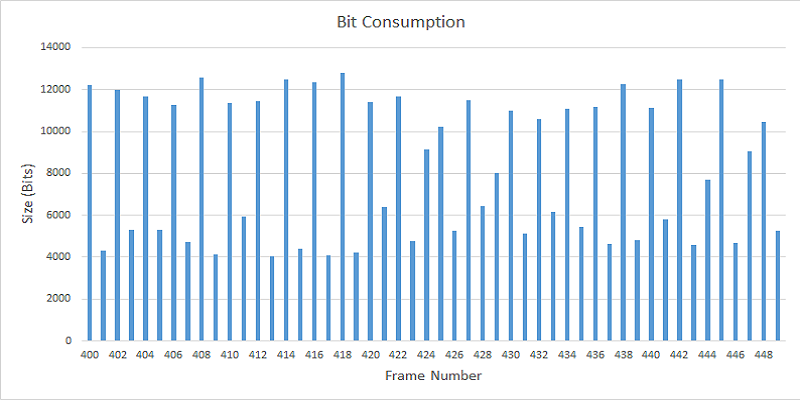
\includegraphics[width=\textwidth]{RC_bit_allocation/Oscillation/Paul250kbps_RC_bit_alloc_osc.png}
		\caption{}
		\label{fig: ROI bit-alloc oscc}
	\end{subfigure}
	\begin{subfigure}[t]{\textwidth}
		\centering
		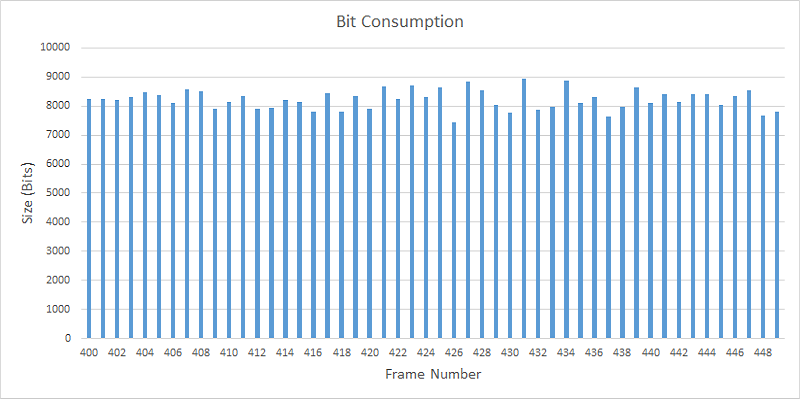
\includegraphics[width=\textwidth]{RC_bit_allocation/Oscillation/Paul250kbps_RC_bit_alloc_corrected_osc.png}
		\caption{}
		\label{fig: ROI bit-alloc oscc corrected}
	\end{subfigure}
	\caption{A plot of frame size in bits for 50 frames from frame number 400 to 450 for the encoded Paul250kbps content with Bit-allocation based ROI encoding. The two figures vary in approach used to update the deviation factors for ROI and non-ROI regions (a) Simultaneous update (b) Alternate Frame Update}
	\label{fig: ROI bit-alloc oscc example}
\end{figure}
%%Results of ROI-based bit-allocation
\begin{figure}
	\centering
	\begin{subfigure}[t]{0.49\textwidth}
		\centering
		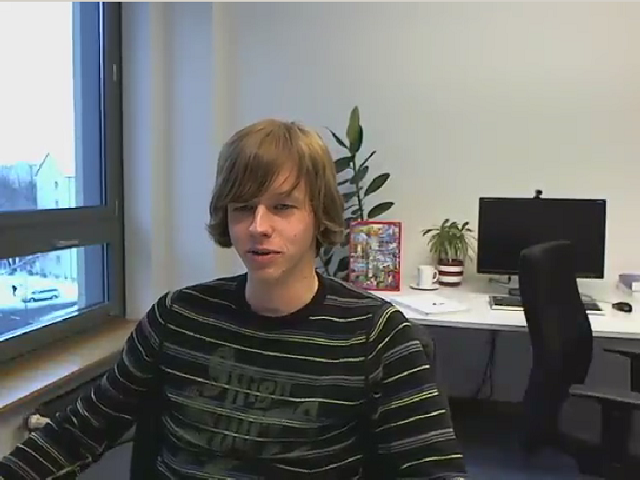
\includegraphics[width=\textwidth]{RC_bit_allocation/Paul250kbps_ROI_bit_alloc.png}
		\caption{}
		\label{fig:ROI bit-allocation result image}
	\end{subfigure}
	\begin{subfigure}[t]{0.49\textwidth}
		\centering
		
\includegraphics[width=\textwidth]{RC_bit_allocation/Paul250kbps_ROI_bit_alloc_psnr_abs45.png}
		\caption{}
		\label{fig:ROI bit-allocation result psnr}
	\end{subfigure}
	\begin{subfigure}[t]{\textwidth}
		\centering
		
\includegraphics[width=0.49\textwidth]{RC_bit_allocation/Paul250kbps_ROI_bit_alloc_quant.png}
		\caption{}
		\label{fig:ROI bit-allocation result quant}
	\end{subfigure}
	\caption{The results of ROI-based encoding using ROI based bit-allocation.(a) Snapshot of encoded video, (b) absolute PSNR map (range 25dB - 50dB), (c) quantization map}
	\label{fig:ROI bit-allocation result}
\end{figure}
\subsubsection{Results}
The bit-allocation based ROI encoding considers input content characteristics to perform the bit-allocation for ROI blocks. Therefore, this approach is applicable to generic contents and hence can be expected to be more robust across multiple contents. The results of this approach is shown in Figure 

The advantages and disadvantages of this approach compared to QP offset approach can be summarized as follows.
\subsubsection*{Advantages}
\begin{itemize}
\item The consideration of input content characteristics for ROI-based encoding makes this approach work well for all types of contents
\item This approach can guarantee minimum quality for the background region by having sufficient bits allocated to the non-ROI to avoid blockiness.
\item The variable importance of ROI can be factored in easily by altering the bias factor (k) to vary the magnitude of bit movement from ROI to non-ROI.
\end{itemize}

\subsubsection*{Disadvantages}
\begin{itemize}
\item This approach requires changes to the bit-allocation module and hence more complex to implement.
\item The determination of relative complexity factor $(C_R)$ needs trained models to predict bit-consumption of ROI and non-ROI parts during normal encoding without using ROI information. This prediction model has bad accuracy for macroblocks encoded with inter prediction. 
\end{itemize}
%
%
%Bibiliography and reference
%
%
%
\clearpage
\begin{thebibliography}{9}
\bibitem{HighQualityROICodingForVideoConferencing} 
Manzur Murshed and James Brown. 
\textit{High Quality Region-of-Interest Coding for Video Conferencing based Remote General Practitioner Training}. 
The Fifth International Conference on eHealth, Telemedicine, and Social Medicine.

\bibitem{ComparingCodingEfficiency} 
J. Ohm. G. J. Sullivan, H. Schwarz, Thiow Keng Tan and T. Wiegand.
\textit{Comparison of the Coding Efficiency of Video Coding Standards—Including High Efficiency Video Coding (HEVC).}
 IEEE Transactions on Circuits and Systems for Video Technology ( Volume: 22, Issue: 12, Dec. 2012 )

\bibitem{JVTF086}
Siwei Ma, Wen Gao, Yan Lu and Hanqing Lu.
\textit{Proposed draft description of rate control on JVT standard. }
Joint Video Team (JVT) of ISO/IEC MPEG and ITU-T VCEG (ISO/IEC JTC1/SC29/WG11 and ITU-T SG16 Q.6) 6h Meeting: Awaji, 5-13, December, 2002.

\bibitem{ROI-Coding-paper}
Manzur Murshed, Md. Atiur Rahman Siddique, Saikat Islam and James Brown.
\textit{High Quality Region-of-Interest Coding for Video Conferencing based Remote General Practitioner Training.}
eTELEMED 2013 : The Fifth International Conference on eHealth, Telemedicine, and Social Medicine

\bibitem{ROI-background-blurring}
A. Cavallaro, O. Steiger, T. Ebrahimi, \textit{"Semantic video analysis for adaptive content delivery and automatic description"}
IEEE Trans. Circuits Syst. Video Technol., vol. 15, no. 10, pp. 1200-1209, Oct. 2005.

\bibitem{Perception-model-of-face}
Mai Xu, Xin Deng, Shengxi Li, \textit{"Region-of-Interest Based Conversational HEVC Coding with Hierarchical Perception Model of Face"}
IEEE Journal of Selected Topics in Signal Processing ( Volume: 8, Issue: 3, June 2014 )

\bibitem{ROI-bit-allocation-h264}
G.-L. Wu, Y.-J. Fu, S.-Y. Chien, \textit{"Region-based perceptual quality regulable bit allocation and rate control for video coding applications"},
Proc. VCIP, 2012.

\bibitem{pre-postprocessig-ROI-codec-independent}
Holger Meuel, Florian Kluger, Jorn Ostermann, \textit{"Codec independent region of interest video coding using a joint pre- and postprocessing framework"}, 
IEEE International Conference on Multimedia and Expo (ICME), July 2016

\bibitem{ROI-MV-based-face-tracking}
Lin Tong, K.R. Rao \textit{"Region of interest based H.263 compatible codec and its rate control for low bit rate video conferencing"}, 
Intelligent Signal Processing and Communication Systems, 2005. ISPACS 2005. Proceedings of 2005 International Symposium on, vol., no., pp. 249- 252, 13-16 Dec. 2005.

\bibitem{InTech-Rate-control-in-video-coding}
Zongze Wu, Shengli Xie1, Kexin Zhang and Rong Wu, \textit{"Rate Control in Video Coding"},
Recent Advances on Video Coding, J. Del Ser Lorente, Ed. InTech,
2011, 79–117. \url{http://www.intechopen.com/books/recent-advances-onvideo-coding/rate-control-in-video-coding}

\bibitem{ROI-aerial-surveillance}
Holger Meuel, Marco Munderloh, Jörn Ostermann, \textit{"Low Bit Rate ROI Based Video Coding for HDTV Aerial Surveillance Video Sequences"}, 
Proc. of the IEEE Conf. on Computer Vision and Pattern Recognition - Workshops (CVPRW), pp. 13-20, June 2011.

\bibitem{foveated-rate-control}
S. Lee, A. C. Bovik, \textit{"Fast algorithms for foveated video processing"},
IEEE Trans. Circuits Syst. Video Technol., vol. 13, no. 2, pp. 149-161, Feb. 2003.

\bibitem{ROI-rate-control-H264}
Fan Li, Na Li, \textit{"Region-of-interest based rate control algorithm for H.264/
AVC video coding"},
Multimed Tools Appl (2016) 75:4163–4186
 
%%Not so Important Reference
\bibitem{human-vision-proof-NSI}
B. Wandell, \textit{"Foundations of Vision"}, 1995, Sinauer.

\bibitem{Leaky-bucket-NSI}
\url{http://www.eenadupratibha.net/pratibha/engineering/content_three_tra_layer_u6.html}
\end{thebibliography}

\subsection{Reaction Factor - Buffer control} 

\begin{figure}[!h]
	\centering
	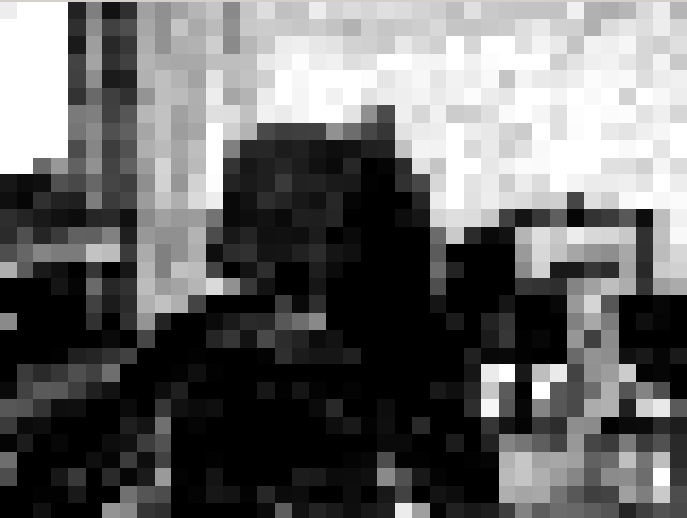
\includegraphics[scale=0.4]{PaulDefault120_91250kbps_psnr}
	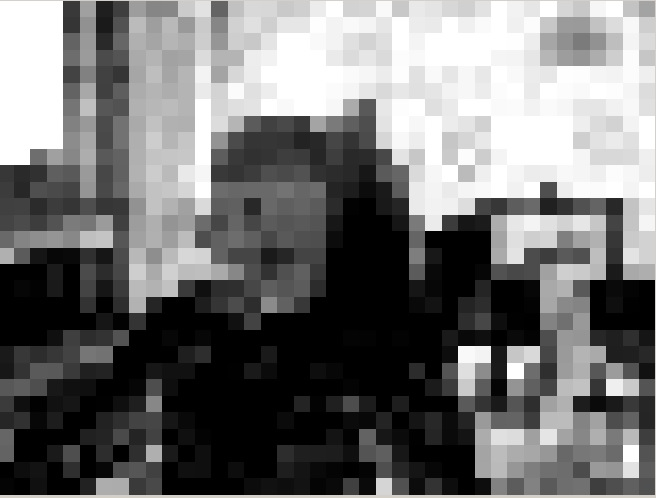
\includegraphics[scale=0.4]{BufferControl/paul120_250kbps_BufferControl_psnr}
	
\includegraphics[scale=0.4]{PaulDefault120_91250kbps}
	
\includegraphics[scale=0.4]{BufferControl/paul120_250kbps_bufferControl}
	
\includegraphics[scale=0.37]{PaulDefault120_91250kbps_quant}
	
\includegraphics[scale=0.4]{BufferControl/paul120_250kbps_BufferControl_quant}    
	\caption{Comparing the images with modified reaction for ROI macroblcoks}
	\label{fig:Default_BufferControlCompare}
\end{figure}
\begin{figure}[!h]
	\centering
	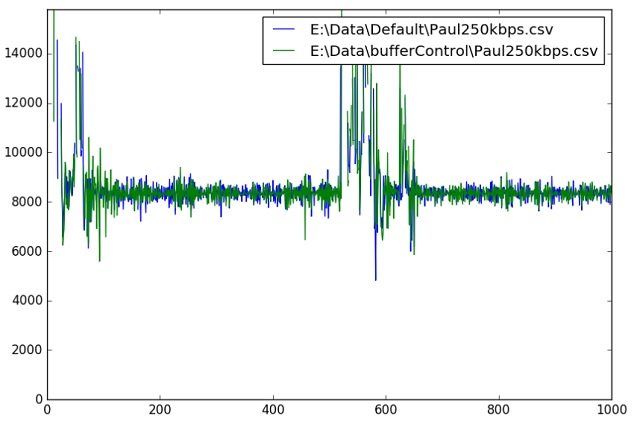
\includegraphics[scale=0.75]{BufferControl/Paul250kbps_Buffer_Control_Delay}
	\caption{Delay Comparison of original video with ROI based reaction factor modification}
	\label{fig:DelayDefault_BufferControltCompare}
\end{figure}
The second approach of using the ROI information to enhance quality of ROI is by using different buffer controls inside the bitrate control module. The bitrate control module used in this study compensates for the overconsumption or underconsumption of bits in the past by adjusting the delta bits during bit allocation of the future frames. This corrected allocation happens at every macroblock level. For instance, if there is excessive consumption of bits in the past macro-blocks, the excess is subtracted from bit budget of certain number of future frames known as reaction factor. If the reaction factor is low, the excess or shortage of bits is shared by a large number of macro-blocks.

The reaction factor is used to allocate additional bits to ROI by using different reaction factors for macro-blocks belonging to the ROI. For instance, in case of underconsumption in the past, the excess bits available for future macroblocks is forced to be used aggressively for macroblocks belonging to ROI. On the other hand whenever there is overconsumption in the past, the bits are reduced more aggressively for macroblocks belonging to non-ROI. The advantage of this approach over QP offset approach is that the bit-allocation is still controlled within the rate control module and its decisions are not overridden by external offsets. This guarantees better buffer compliance. The results shown in Figure \ref{fig:Default_BufferControlCompare} compares the output with modified reaction factor based on region of interest and original video. It can be noticed that PSNR of the face regions is very close to that of the background. The data in Table \ref{AllPSNR1} shows that PSNR of ROI region is actually higher than the overall frame PSNR. The delay plots in \ref{fig:DelayDefault_BufferControltCompare} shows there is no significant changes in the delay or bitrate consumption.

\end{document}